% !TEX root = ../main.tex
%
%\begin{savequote}[8cm]
%	Everyone by now presumably knows about the danger of premature optimization. 
%	I think we should be just as worried about premature design - 
%	designing too early what a program should do.
%	\qauthor{--- Paul Graham}
%\end{savequote}

\chapter{Automating Learning -- Bayesian Optimization for Probabilistic Programs}
\label{chp:bopp}

% !TEX root =  ../main.tex

So far in this thesis, and in the literature more generally, the focus has been on automating
inference for probabilistic programs.  However, as we explained in Section~\ref{sec:opt:intro},
optimization is also a very important tool in the machine learning toolbox.  Further, many problems
require concurrent inference and optimization in the form of marginal maximum a posteriori (MMAP) estimation,
maximum marginal likelihood (MML) estimation, or risk minimization.  In this chapter, we develop a probabilistic programming framework
for automating the solution of these mixed inference-optimization problems.
We will focus for the most part on
MMAP estimation, highlighting differences for MML estimation and risk minimization when necessary.

MMAP estimation is challenging as it corresponds to the optimization of an intractable integral, such that the 
optimization target is expensive to evaluate and gives noisy results.  Current PPS inference engines are 
typically unsuited to such settings.  We therefore introduce BOPP\footnote{Code available at \url{http://www.github.com/probprog/bopp/}}
(Bayesian optimization for probabilistic programs)~\citep{rainforth2015workshopbopp,rainforth2016bayesian}, 
which uses a series of code transformations, existing inference algorithms,
and a bespoke Gaussian process (GP) based Bayesian optimization (BO) package, which we call Deodorant\footnote{Code available
at \url{http://www.github.com/probprog/deodorant/}}, to optimize the evidence of a query with respect to
an arbitrary subset of its internally sampled variables.\footnote{As we will explain later, there is no need to
	provide separate consideration for optimizing with respect to the inputs of the query as, if required,
	variables can be trivially internalized.}

BOPP can be viewed from two different perspectives, providing distinct contributions to both the probabilistic
programming and Bayesian optimization literatures.  From a probabilistic programming perspective, we can
view BOPP as extending PPSs beyond their typical inference setting to a more
general mixed inference-optimization framework.  It allows users to specify a model in the same manner 
as existing systems, but then select some subset of the sampled variables in the query to be optimized, 
with the rest marginalized out using existing inference algorithms.  Though the exact code transformations we
introduce are inevitably language specific and have been implemented for Anglican, the concepts we
introduce apply more widely and the BO package itself, Deodorant, is not PPL specific and is provided
as a stand-alone package.  More generally, the \textit{optimization query} we 
introduce can be implemented and utilized in any PPL that supports an inference method returning a 
partition function estimate.  This framework increases the scope of models that can be expressed in
PPSs and gives additional flexibility in the outputs a user can request from a program.

From a BO perspective, we can view BOPP as the first package to directly exploit the source code of its target.
This leads to a number of novel contributions to the BO literature, such as innovations in 
problem-independent hyperpriors, unbounded optimization, and implicit constraint satisfaction.  
The ability to do these is rooted
in the ability provided by PPLs to manipulate the target source code and return artifacts suitable for carrying
out certain tasks on a model.  For example, we use a code transformation to produce a problem-specific
optimizer for the acquisition function that ensures the implicit constraints specified by the query,
including equality constraints not before considered by the BO literature, are automatically and exactly
satisfied.  As a consequence, BOPP provides a significant novel features and performance
improvements even when used simply as a conventional BO package.

\section{Motivation} 
\label{sec:IntroductionBOPP}

% !TEX root =  ../main.tex

\todo[inline]{Move this first paragraph to the prob prog section to make a better opening}

Probabilistic programming systems (PPS) allow probabilistic models to be represented in the form of a generative model and statements for conditioning on data \citep{carpenter2015stan,goodman_uai_2008,goodman_book_2014,mansinghka2014venture,minka_software_2010,wood2014new}.  
%Informally, one can think of the generative model as the definition of a prior, the conditioning statements as the definition of a likelihood and the output of the program as samples from a posterior distribution. 
Their core philosophy is to decouple model specification and inference, the former corresponding to the user-specified program code and the latter to an inference engine capable of operating on arbitrary programs.  Removing the need for users to write inference algorithms significantly reduces the burden of developing new models and makes effective statistical methods accessible to non-experts.
%This inference engine must therefore be general purpose and robust, without making strong assumptions about the structure of the program, often taking the form of a Monte Carlo sampling scheme such as Markov chain Monte Carlo (MCMC) \citep{wingate2011lightweight}, Hamiltonian Monte Carlo \citep{carpenter2015stan}, sequential Monte Carlo (SMC) \citep{wood_aistats_2014} or particle MCMC \citep{van2015particle}.  

Although significant progress has been made on the problem of general purpose \emph{inference} of program variables, less attention has been given to their \emph{optimization}.  Optimization is an essential tool for effective machine learning, necessary when the user requires a single estimate. It also often forms a tractable alternative when full inference is infeasible \citep{murphy2012machine}.  Moreover, coincident optimization and inference is often required, corresponding to a marginal maximum a posteriori (MMAP) setting where one wishes to maximize some variables, while marginalizing out others.  Examples of MMAP problems include hyperparameter optimization, expectation maximization, and policy search \citep{van2015black}.

%Here pure optimization, i.e. assuming the best possible possible environment, is clearly unsatisfactory, whilst inference alone is insufficient to determine the optimal action.

%Although significant progress has been made on the problem of general purpose \emph{inference} of program variables, less attention has been given to their \emph{optimization}. In many machine learning problems one might want to perform marginal maximum a posterior (MMAP) estimation to obtain a point estimate for a subset of random variables in a model while marginalizing over the remaining variables. Examples of such settings include hyperparameter optimization, decision making under uncertainty \cite{van2015black}, and problems where inference over top-level variables is either infeasible or the user simply desires a single point estimate \cite{murphy2012machine}.

%Even when these simulations are deterministic, this is an approximation to a truly probabilistic world. This setting corresponds to a MMAP framework, in which the user wishes to select the best design whilst marginalizing out the uncertainty about the environment or the simulation itself.

%To demonstrate how easily BOPP can be used, we present an application of optimal power allocation is shown in Figure \ref{fig:houses} with associated code in Figure \ref{fig:house-heating-code}.  Typically an engineer might try to solve this problem by making a number of fixed environmental assumptions and invoking a finite element simulation software, tuning by hand.  This process can be laborious and fails to capture the uncertainty in the environment.  BOPP provides a framework to naturally incorporate these uncertainties, whilst still exploiting the original simulation and returning a single solution the engineer can implement.

%In this paper we develop the first system that extends probabilistic program (PP) inference to a more general MMAP framework, wherein the user specifies a model in the same manner as existing systems, but then selects some subset of the sampled variables in the program to be optimized, with the rest marginalized using existing inference algorithms.  To do so, we define an \emph{optimization query}, which performs a program transformation to map unconditioned random variables onto conditioned random variables, whose values are passed to the transformed program as inputs. We then introduce Bayesian optimization for probabilistic programs (BOPP), a new framework for Gaussian process (GP) \citep{rasmussen2006gaussian} based  Bayesian optimization (BO) \citep{osborne2009gaussian, jones1998efficient} package integrated into the PPS Anglican \citep{wood2014new}. The BOPP method iteratively performs inference in a conditioned program using a generic method, such as sequential Monte Carlo (SMC), to obtain an unbiased estimate of the marginal likelihood of a conditioned program. Bayesian optimization of this marginal likelihood is then done by constructing a GP surrogate and maximizing the expected improvement \cite{brochu2010tutorial} to select values in a manner that balances exploration and exploitation. 

In this paper we develop the first system that extends probabilistic programming (PP) to this more general MMAP framework, wherein the user specifies a model in the same manner as existing systems, but then selects some subset of the sampled variables in the program to be optimized, with the rest marginalized out using existing inference algorithms.  The \textit{optimization query} we introduce can be implemented and utilized in any PPS that supports an inference method returning a marginal likelihood estimate.  This framework increases the scope of models that can be expressed in PPS and gives additional flexibility in the outputs a user can request from the program.

MMAP estimation is difficult as it corresponds to the optimization of an intractable integral, such that the optimization target is expensive to evaluate and gives noisy results.  Current PPS inference engines are typically unsuited to such settings.  We therefore introduce BOPP\footnote{Code available at \href{http://www.github.com/probprog/bopp/}{\url{http://www.github.com/probprog/bopp/}} \vspace{7pt}} 
(Bayesian optimization for probabilistic programs) which couples existing inference algorithms from PPS, like \emph{Anglican} \citep{wood2014new}, with a new Gaussian process (GP) \citep{rasmussen2006gaussian} based Bayesian optimization (BO) package \citep{gutmann2016bayesian, jones1998efficient, osborne2009gaussian, shahriari2016unbounded}.  

To demonstrate the functionality provided by BOPP, we consider an example application of engineering design.  Engineering design relies extensively on simulations which typically have two things in common: the desire of the user to find a single best design and an uncertainty in the environment in which the designed component will live. Even when these simulations are deterministic, this is an approximation to a truly stochastic world. By expressing the utility of a particular design-environment combination using an approximate Bayesian computation (ABC) likelihood \citep{csillery2010approximate}, one can pose this as a MMAP problem, optimizing the design while marginalizing out the environmental uncertainty.

\flushbottom

\begin{figure*}[t]
	%\includegraphics[width=\textwidth]{"figures/house-heating/deterministic/house-heating-deterministic-with-convergence"}
	\centering
	\begin{subfigure}[t]{0.47\textwidth}
		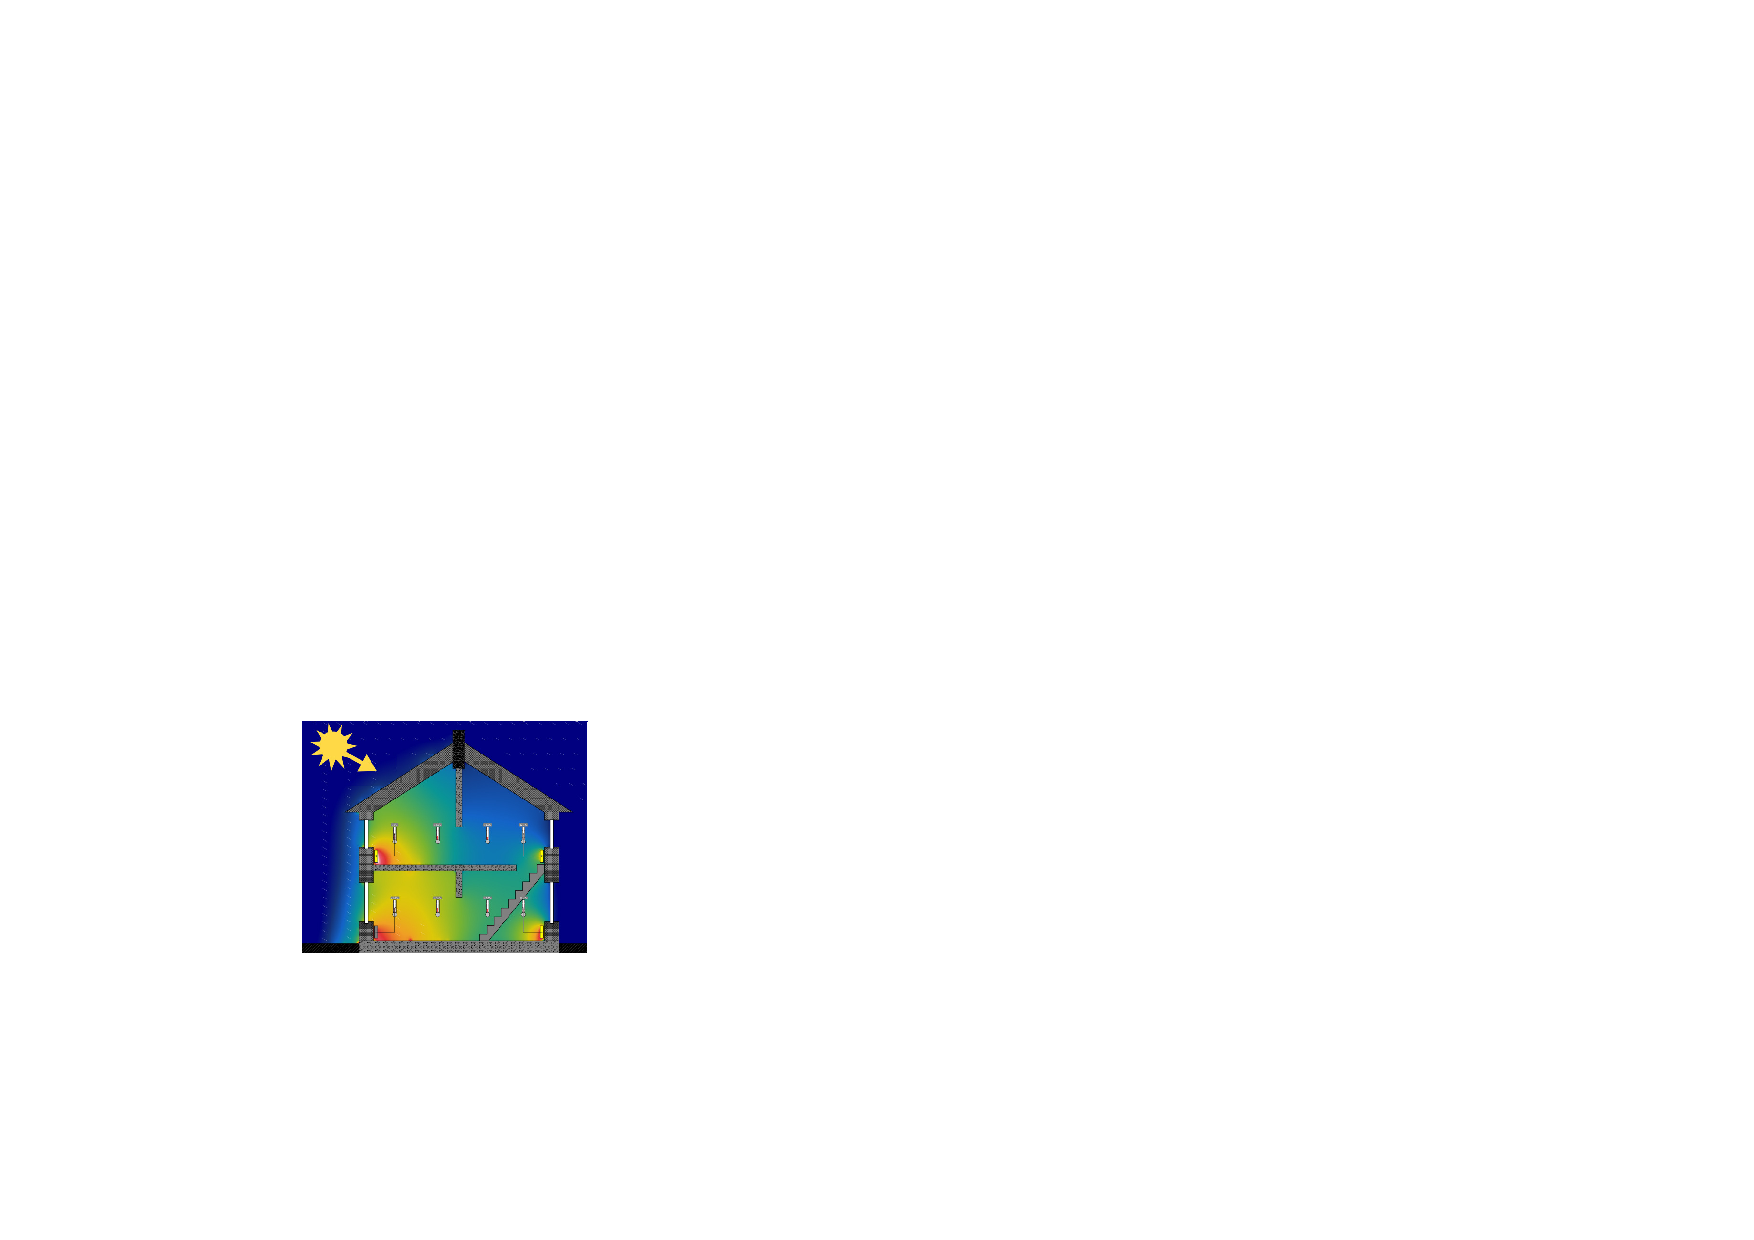
\includegraphics[width=\textwidth]{house-heating/even_powers.pdf}
		\caption{Radiator powers set evenly}
	\end{subfigure}
	~~~~ %\hspace{40pt}
		\begin{subfigure}[t]{0.47\textwidth}
			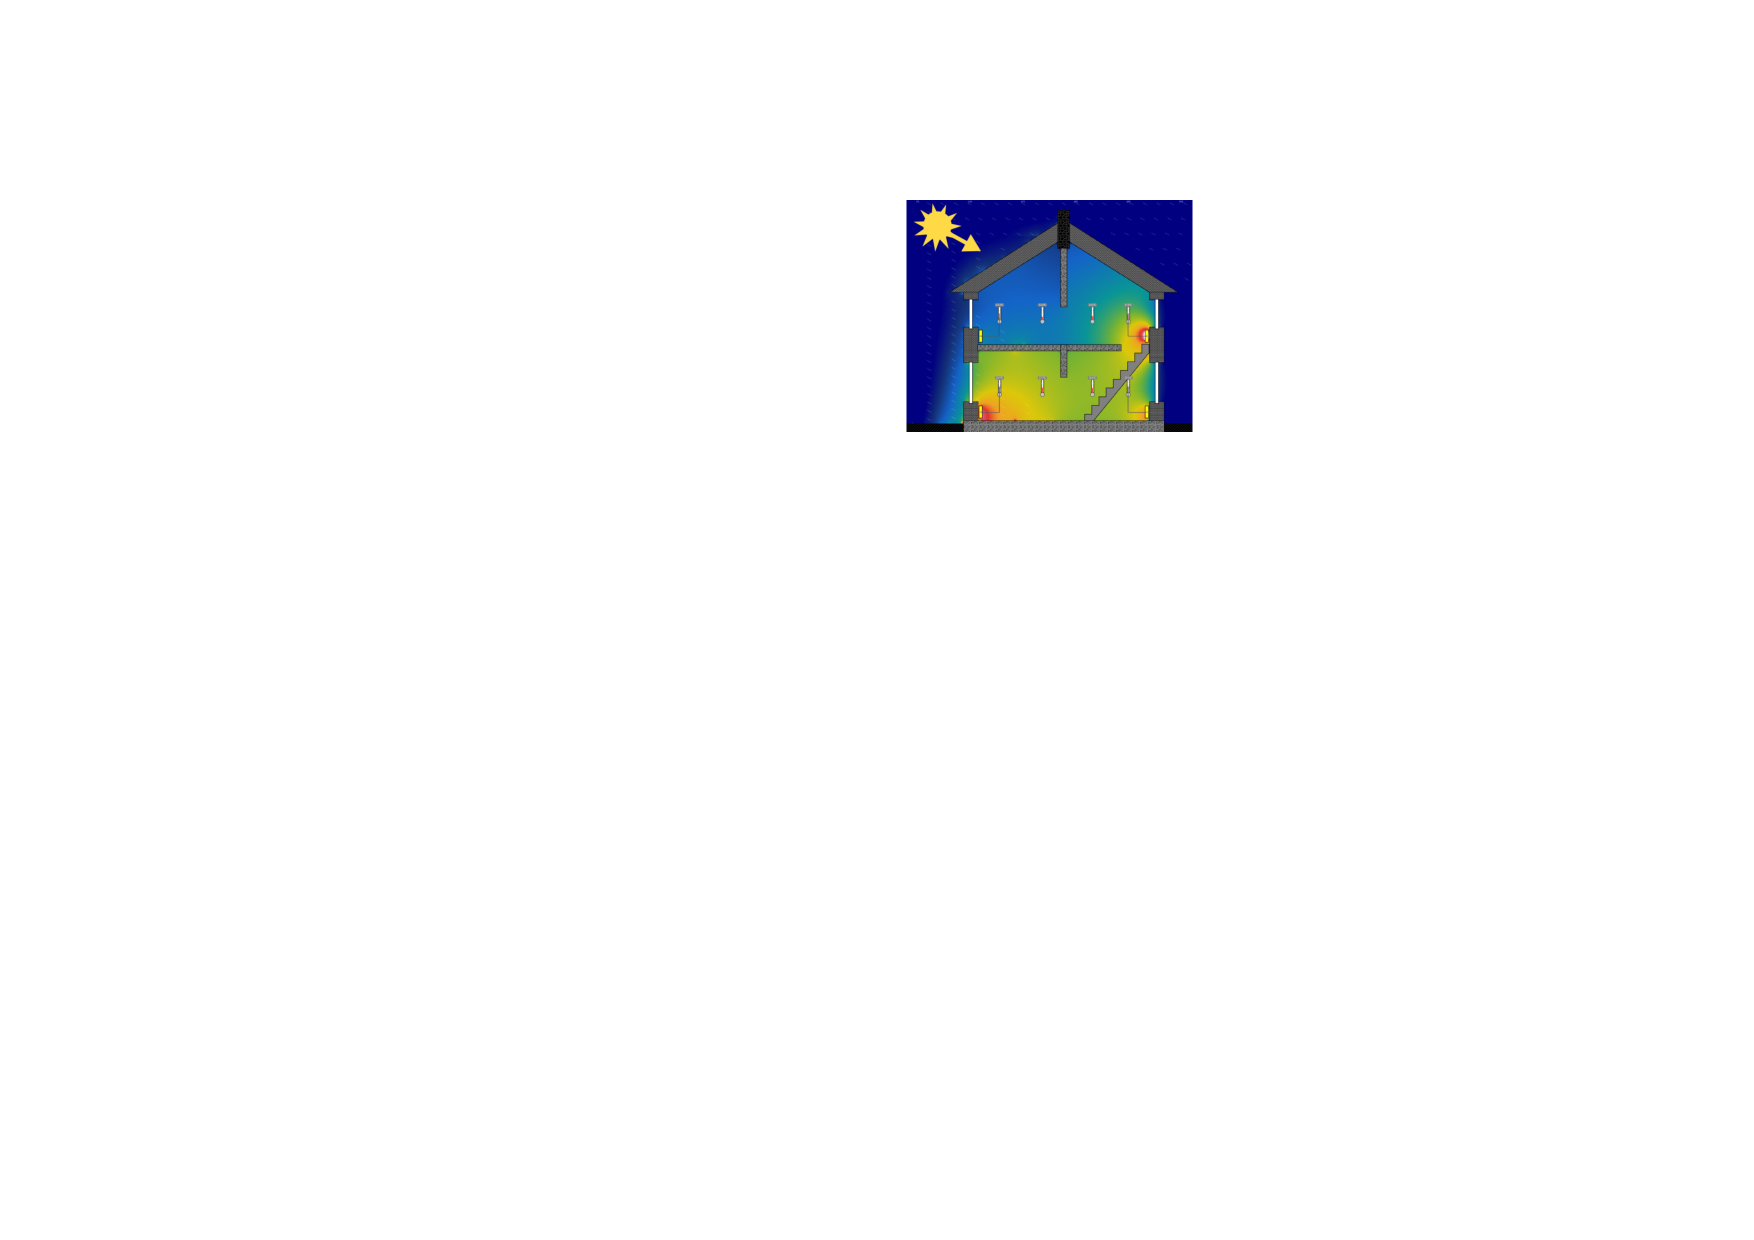
\includegraphics[width=\textwidth]{house-heating/first_iter.pdf}
			\caption{Best setup from BOPP initialization}
		\end{subfigure} \\
		\vspace{10pt}
			\begin{subfigure}[t]{0.47\textwidth}
				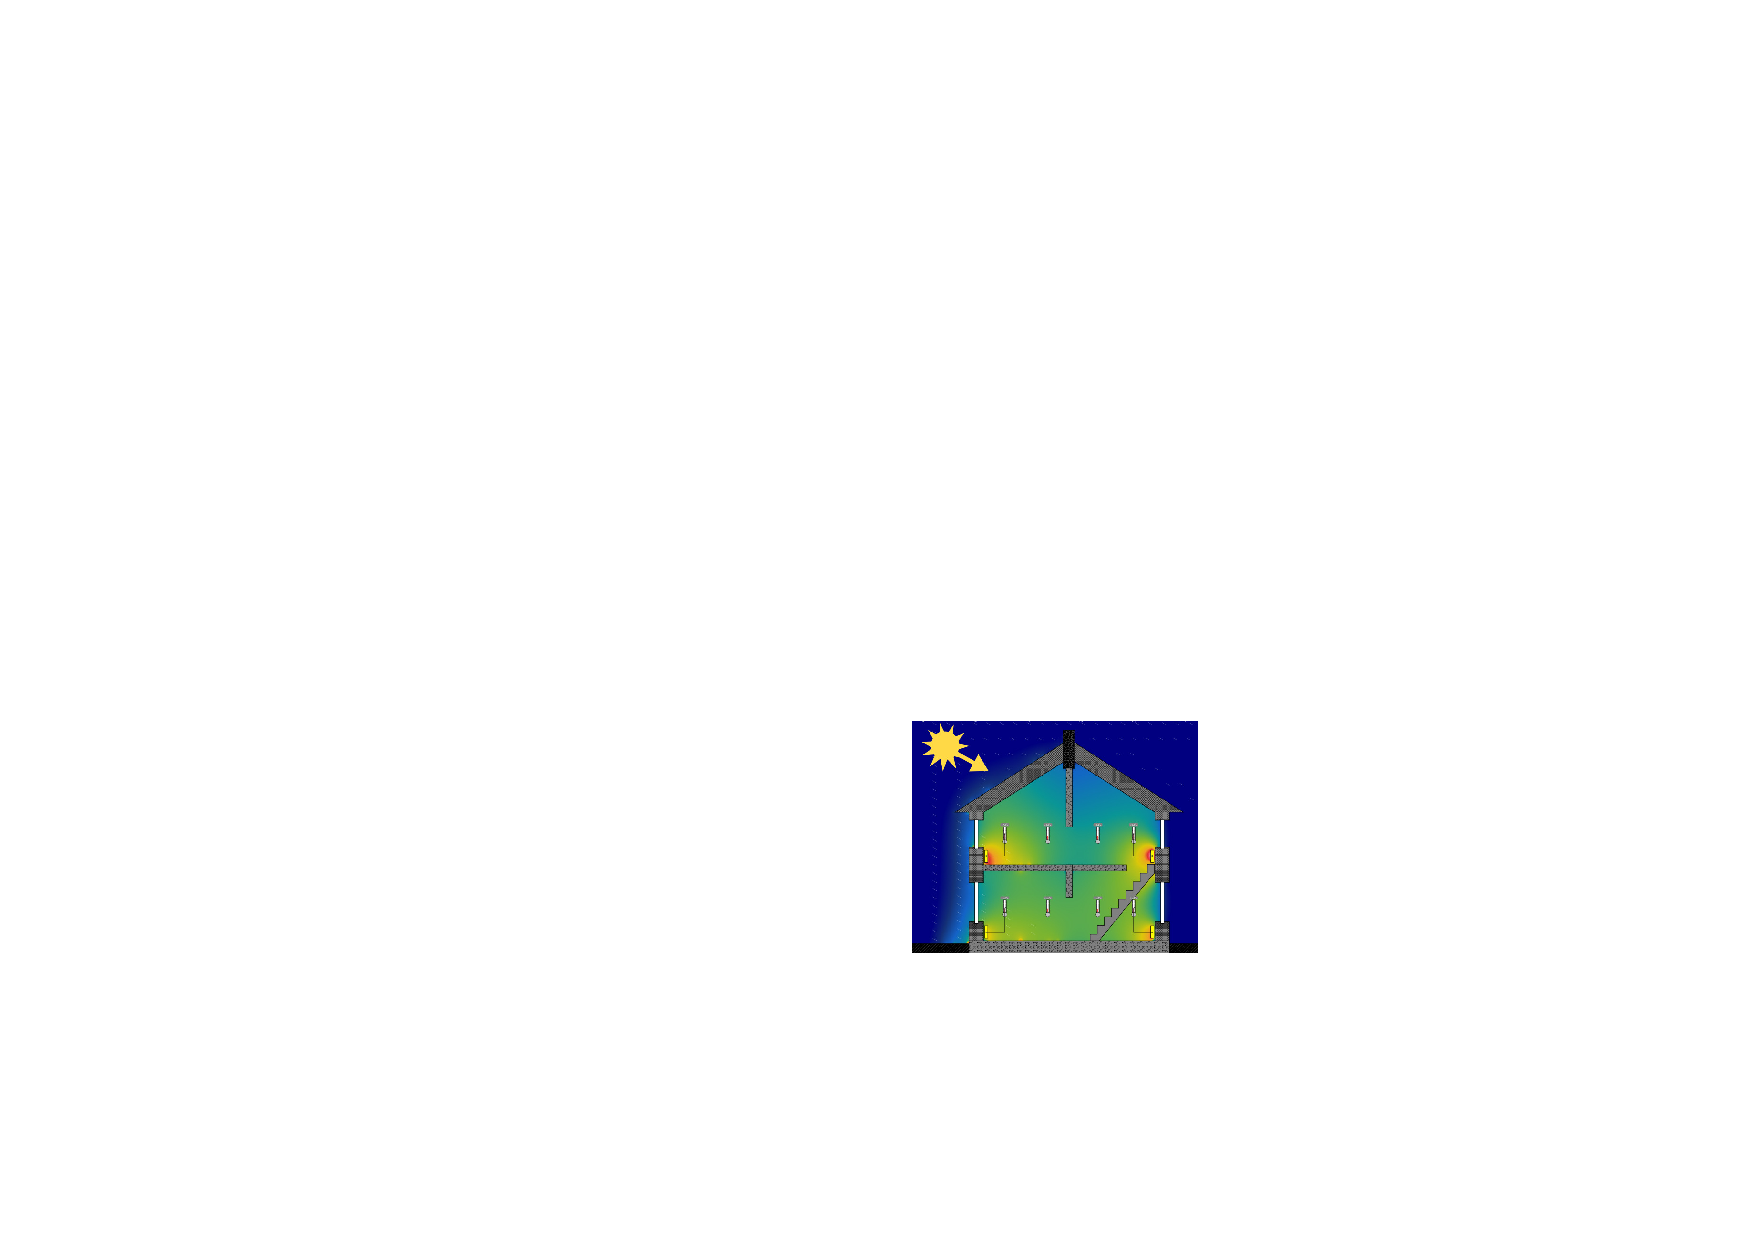
\includegraphics[width=\textwidth]{house-heating/100_iters.pdf}
				\caption{Best setup after 100 iterations of BOPP}
			\end{subfigure}
		~~~~ %	\hspace{40pt}
			\begin{subfigure}[t]{0.47\textwidth}
				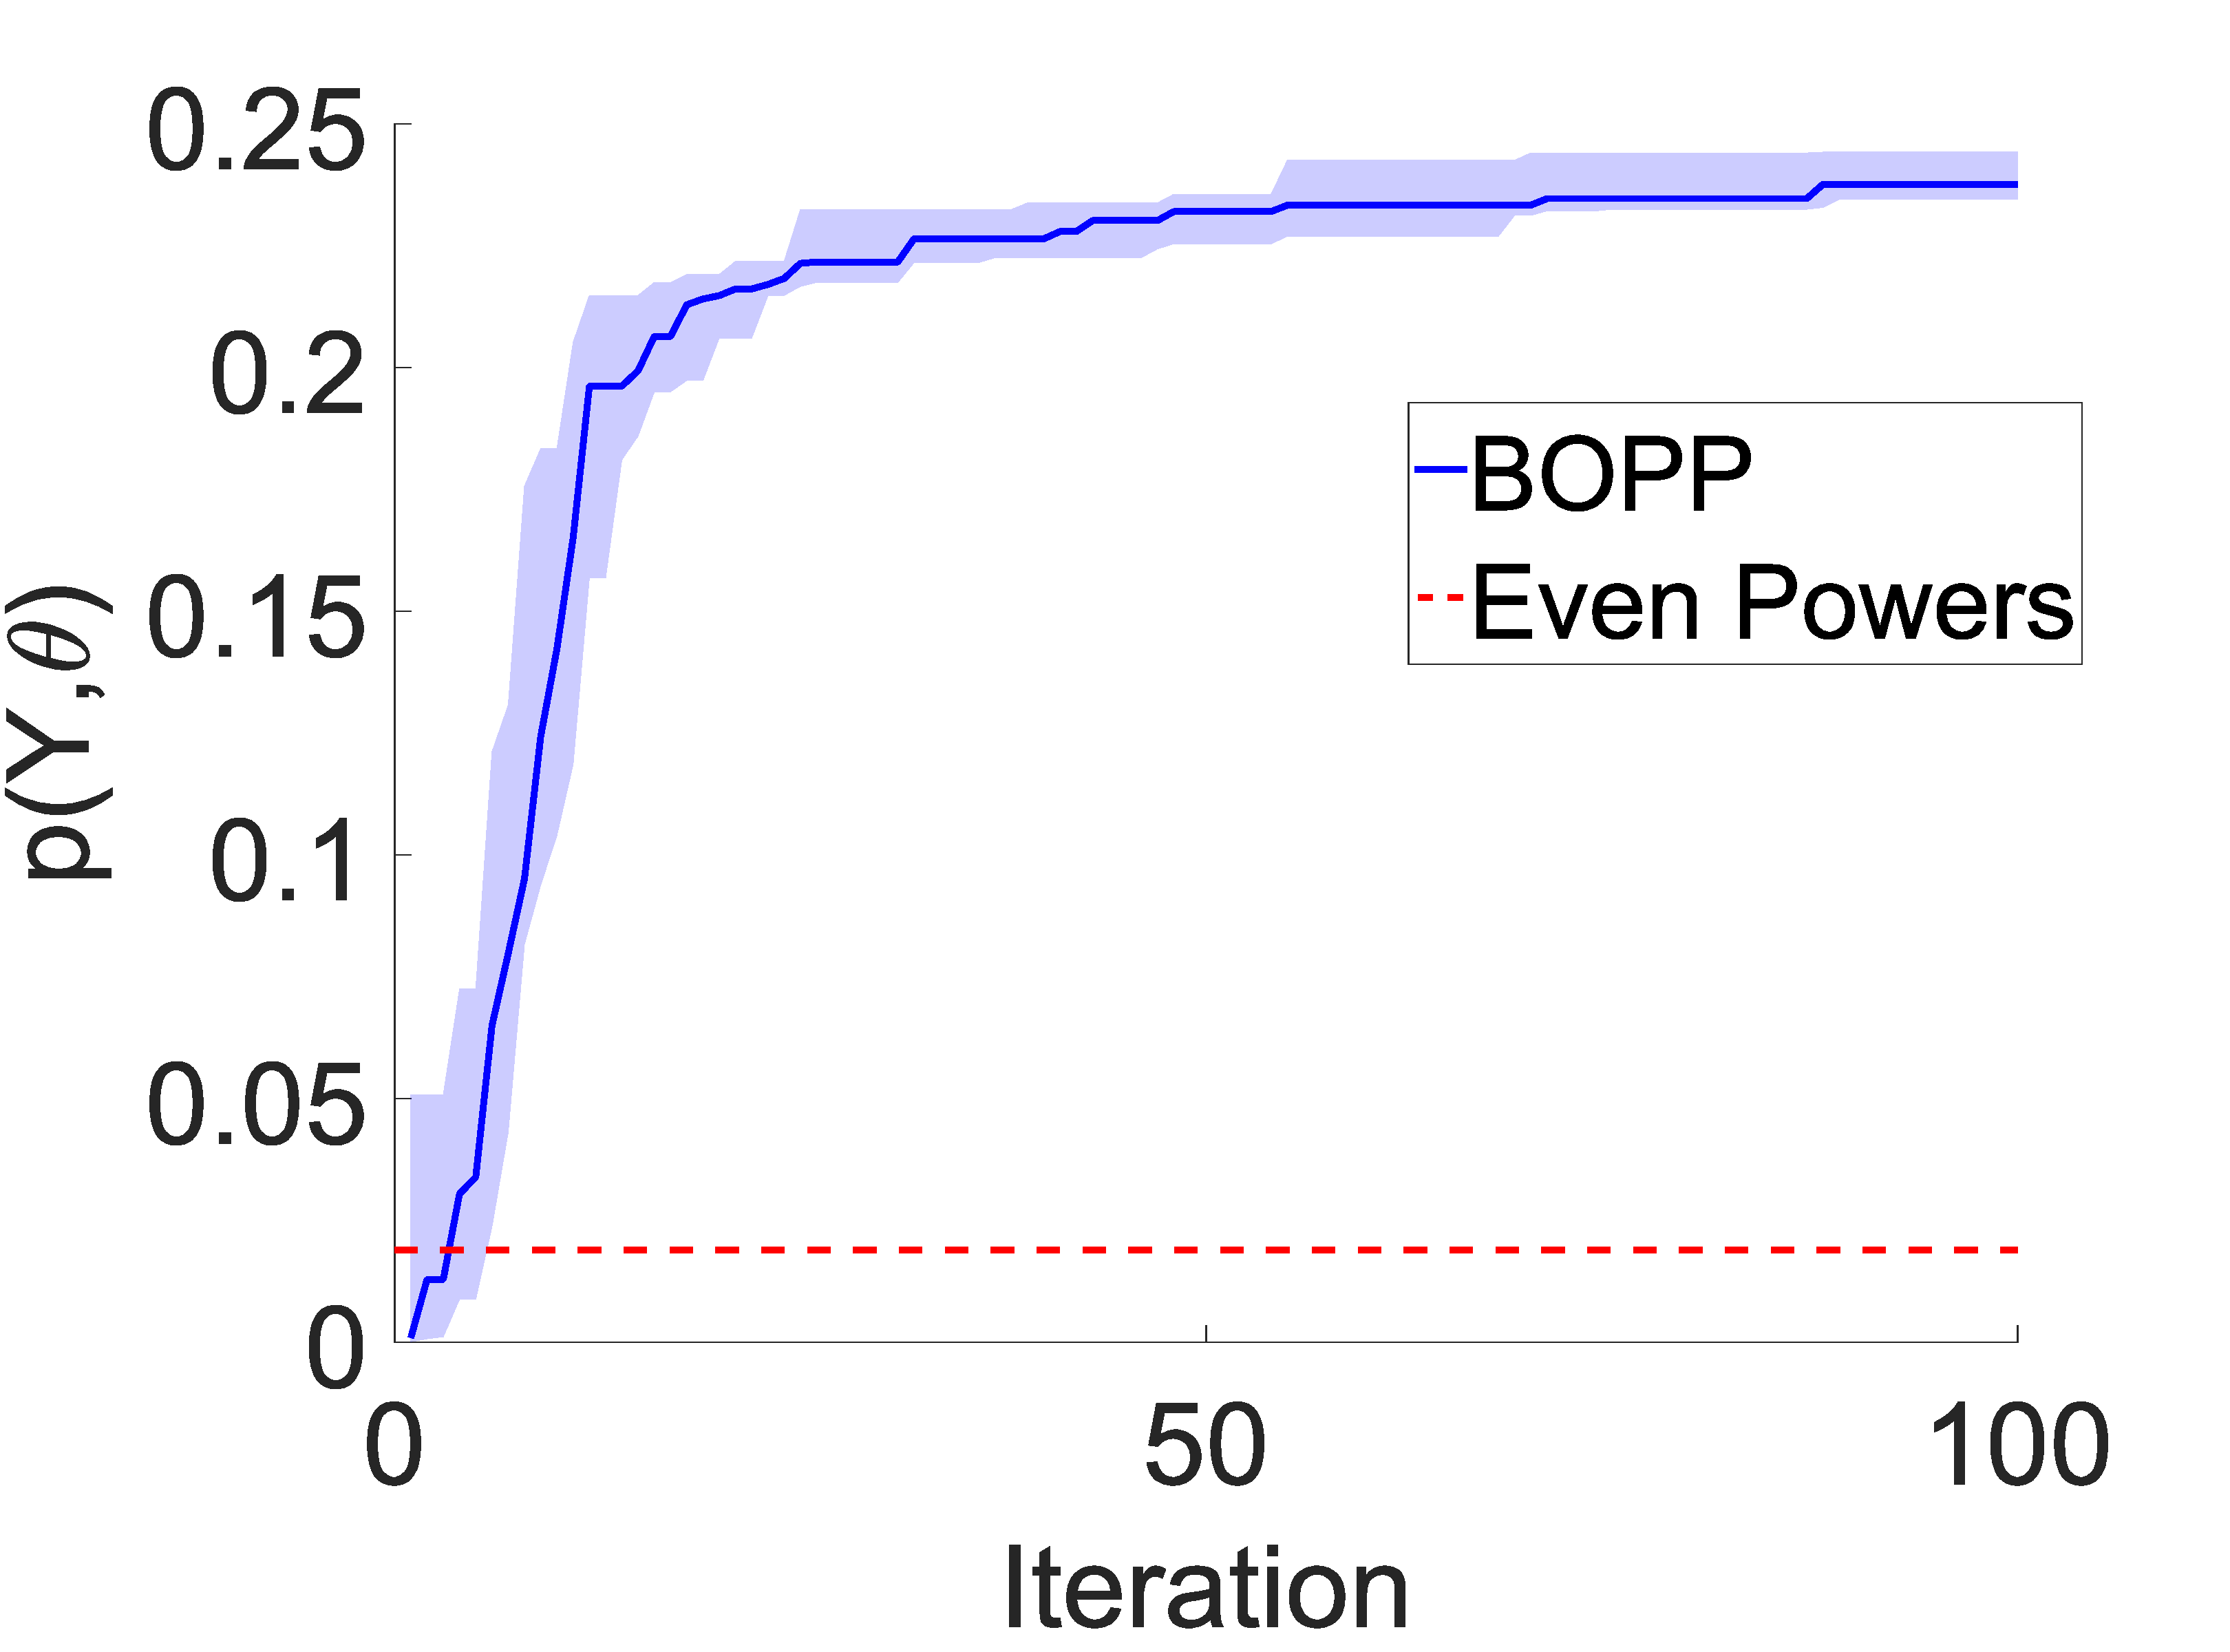
\includegraphics[width=\textwidth]{house-heating/heating_rerun.pdf}
				\caption{Convergence of evidence}
			\end{subfigure}
	% \centering ~~~
	% \includegraphics[width=0.24\textwidth]{"figures/house-heating/probabilistic/logZ-with-even-redblue-wide"}
	%			\caption{
	%				\label{fig:houses-convergence}
	%				Log marginal likelihood $\log Z$ for the \lsi{house-heating} query in Figure~\ref{fig:house-heating-code}. 
	%			}
	%	
	\caption{
		\label{fig:houses}
		Simulation-based optimization of radiator powers subject to varying solar intensity. Shown are output heat maps from Energy2D \citep{xie2012energy2d} simulations at one intensity, corresponding to setting all the radiators to the same power (\emph{top left}), the best result from a set of 5 randomly chosen powers used for initializing BOPP (\emph{top right}), and the best setup found after 100 iterations of BOPP (\emph{bottom left}). The bottom right plot shows convergence of the evidence of the respective model, giving the median and 25/75\% quartiles.
		%Simulation-based optimization of the radiator power subject to varying solar intensity. Here (a-c) show output heat maps from Energy2D \citep{xie2012energy2d} simulations, corresponding respectively to setting all the radiators to the same power, the best result from a set of randomly chosen initializations and the best setup found after 100 iterations of BOPP. (d) shows convergence of the evidence of the respective model as a function of simulation evaluations for independent restarts.
		%Homogenizing the temperature of a 2D model of a house using BOPP. The house has four adaptively controlled radiators, with additional uneven eating is provided by the sun, which will vary both temporally and probabilistically.  Our aim is to select the base power for each of the radiators, subject to some total energy budget, whilst marginalizing out the different anticipated weather conditions.  To do this, the BOPP query given in Figure \ref{fig:house-heating-code} wraps around the finite element heat transfer simulation engine Energy2D \citep{xie2012energy2d} and performs the required MMAP estimation. The na\"ive strategy of setting the power densities of the radiators uniformly (\emph{far left}) leads to an uneven heating\protect\footnotemark, noting that the colormap on the top indicates temperature of air from $5^{\circ}\mathrm C$ to $35^{\circ}\mathrm C$.  
		%After a single iteration of BOPP (\emph{middle left}), the found solution is also poor, but after 100 iterations (\emph{middle right}), a significantly improved solution has been achieved.  The log marginal likelihood in terms of iterations of number of heating setups tested is shown (\emph{far right}) for five separate BOPP runs, along with the resulting marginal likelihood from na\"ively setting the radiators to the same power.
		%Imagine that we have a number of rooms each containing a heating element and we wish to optimize the relative powers of the heaters to deliver the most uniform heating of the house over its lifetime given some total energy budget.  
		% For example, the sun will apply uneven heating to house in a manner which various over time, e.g. due to weather changes and variations in the arc of the sun through the year.  BOPP provides a basis to naturally incorporate these uncertainties into the model, whilst still exploiting the original finite element simulation and returning a single solution the engineer can the go implement.  We therefore believe that in the long term, PPS supporting MMAP have the potential to revolutionise the manner in which engineering simulation is approached by incorporating uncertainty from all stages of the process into a single unified framework, reducing the reliance on fudge-factors and educated guesswork.
	}
\end{figure*}

\begin{figure}[tb]
	\begin{lstlisting}[basicstyle=\ttfamily\small]
(defopt house-heating [alphas target-temperatures] [powers]
 (let [solar-intensity (sample weather-prior)
       powers (sample (dirichlet alphas))
       temperatures (simulate solar-intensity powers)]
  (observe (abc-likelihood temperatures) target-temperatures)))
	\end{lstlisting}	
	\vspace{-6pt}
	\caption{BOPP query for optimizing the power allocation to radiators in a house.  Here \lstinline{weather-prior} is a distribution over the solar intensity and a uniform Dirichlet prior with concentration \lsi{alpha} is placed over the powers. Calling \simulatec performs an Energy2D simulation of house temperatures. The utility of the resulting output is incorporated using \abcl, which measures a discrepency from the \texttt{target-temperatures}. Calling \doopt on this query invokes the BOPP algorithm to perform MMAP estimation, where the second input \lstinline{powers} indicates the variable to be optimized. \label{fig:house-heating-code}}
\end{figure}

Figure~\ref{fig:houses} illustrates how BOPP can be applied to engineering design, taking the example of optimizing the distribution of power between radiators in a house so as to homogenize the temperature, while marginalizing out possible weather conditions and subject to a total energy budget. The probabilistic program shown in Figure~\ref{fig:house-heating-code} allows us to define a prior over the uncertain weather, while conditioning on the output of a deterministic simulator (here Energy2D \citep{xie2012energy2d}-a finite element package for heat transfer) using an ABC likelihood.  BOPP now allows the required coincident inference and optimization to be carried out automatically, directly returning increasingly optimal configurations. 

BO is an attractive choice for the required optimization in MMAP as it is typically efficient in the number of target evaluations, operates on non-differentiable targets, and incorporates noise in the target function evaluations.  However, applying BO to probabilistic programs presents challenges, such as the need to give robust performance on a wide range of problems with varying scaling and potentially unbounded support.  Furthermore, the target program may contain unknown constraints, implicitly defined by the generative model, and variables whose type is unknown (i.e. they may be continuous or discrete).

On the other hand, the availability of the target source code in a PPS presents opportunities to overcome these issues and go beyond what can be done with existing BO packages.  BOPP exploits the source code in a number of ways, such as optimizing the acquisition function using the original generative model to ensure the solution satisfies the implicit constaints, performing adaptive domain scaling to ensure that GP kernel hyperparameters can be set according to problem-independent hyperpriors, and defining an adaptive non-stationary mean function to support unbounded BO. 

Together, these innovations mean that BOPP can be run in a manner that is fully black-box from the user's perspective, requiring only the identification of the target variables relative to current syntax for operating on arbitrary programs. We further show that BOPP is competitive with existing BO engines for direct optimization on common benchmarks problems that do not require marginalization.

%that can be implemented in any PPS where inference methods return marginal likelihood estimates. 



%MMAP estimation is generally difficult as it corresponds to the optimization of an intractable integral, such that function evaluations are expensive and give noisy results.  Current PPS inference engines are typically unsuited to such optimization.  We therefore introduce BOPP (Bayesian optimization for probabilistic programs) which couples existing inference algorithms with a new Gaussian process (GP) \citep{rasmussen2006gaussian} based Bayesian optimization (BO) \citep{osborne2009gaussian, jones1998efficient} package integrated into the PPS Anglican \citep{wood2014new}.  



%MMAP estimation for PPS presents further issues such as the need to be general purpose and robust, whilst dealing with potentially unknown constraints defined implicitly within the generative model.  


%On the other hand, the availability of the target source code in PPS presents opportunities to overcome these issues and go beyond what can be done with existing BO packages.  For example, it allows operation under unknown \emph{equality} constraints and applies automatic domain scaling for problem-independent GP hyperpriors.  In addition to delivering improved performance over prominent BO packages when used simply as an optimizer, these innovations mean that BOPP can be run in a manner that is fully black-box from the user's perspective, requiring only the identification of the target variables relative to current syntax for operating on arbitrary programs.

%\footnotetext{Though results are from the full BOPP implementation with sun heating marginalized out, the simulation plots correspond to a single common condition for the sun for visualization purposes.}

%\section{Motivating Example}
%\label{sec:motivation}


%The rest of this paper is outlined as follows: we first provide background on PPS, BO and GPs.  We define a framework for an optimization query and introduce our core code transformation to allow an arbitrary program to be optimized with respect to parameters defined within the program.  Our algorithm for optimizing the evidence of this program using BO and additional code transformations is outlined, we present experiments demonstrating the applicability of our method and we finish with concluding discussions and suggestions for future work.


\section{Related Work} 
\label{sec:bopp:related}

Reasonable consideration has been given before to solving maximum likelihood and marginal 
a posteriori (MAP) problems with PPSs and many systems provide some form of appropriate
estimation scheme (see e.g.~\citep{carpenter2015stan,salvatier2016probabilistic}).  One simple
approach is to apply an annealing to the \observe densities (for maximum likelihood estimation)
or both the \sample and \observe densities (for MAP estimation) in
a conventional MCMC sampler such as LMH (see Section~\ref{sec:proginf:str:lmh}).
This results in a simulated annealing~\citep{aarts1988simulated} algorithm for general purpose programs.
An alternative approach, introduced by~\cite{tolpin-socs-2015}
instead uses ideas from Monte Carlo tree search to construct a general purpose MAP estimator.
However, all of these approaches to not permit the more challenging scenario
where the target is to optimize a marginal distribution.  They are, therefore, not suitable for combined
inference and optimization problems.

One approach that does consider optimization of marginal probabilities of probabilistic
programs is given by~\cite{vandemeent2016black}, which thus perhaps presents the closest
approach to our own work.  The aim of~\cite{vandemeent2016black} is, on the surface, somewhat
different to our own as they look to automate policy search problems~\citep{deisenroth2013survey}
using probabilistic programs.  However, policy search is a particular instance of MML estimation
and so falls within our general problem class.  Moreover, their approach of maximizing an ELBO~\citep{blei2016variational}
using stochastic gradient ascent~\citep{robbins1951stochastic} is, in principle, substantially
more general than policy search problems and constitutes a general MML estimation scheme in its own right.
However, the approach has a number of restrictions and assumptions stemming from its variational 
inference roots.  Perhaps the most critical for our purposes is that gradients are estimated using
importance sampling and thus will generally become increasingly noisy as the dimensionality of the nuisance variables (i.e. those we wish to marginalize over) increases.
The approach also requires mean field approximations
to be made, the appropriateness of which will vary from problem to problem, while, as with other
stochastic gradient ascent approaches, a large number of optimization iterations is typically required
to reach convergence, which can be prohibitive for some problems.  BOPP, on the other hand, requires
very few assumptions to be made and is free to use more advanced inference approaches, for example
SMC, for estimating the marginal likelihood.  One consequence of this is that it can scale to far
higher dimensions in the nuisance variables.  For example, our chaos model in Section~\ref{sec:bopp:exp}
marginalizes over a 1500 dimensional space.

Another interesting alternative approach,
developed since publication of BOPP, involves taking derivatives \emph{through} an SMC
sweep~\citep{le2017auto,naesseth2017variational,maddison2017filtering}. 
More precisely, these methods allow the derivative of the marginal likelihood estimate (or more typically
its logarithm) to be calculated during an SMC sweep, for example by using automatic differentiation
on the calculation of the original estimate~\citep{le2017auto}.  This can be used for MML or MMAP estimation
of global parameters by using these gradients as input to a stochastic gradient ascent scheme.
A key difference of this approach, to say~\cite{vandemeent2016black}, is that using SMC instead of importance
sampling means that substantially lower variance gradient estimates can be achieved.
Though, to the best of our knowledge, no such approach is currently implemented in a PPS, doing so is 
in theory perfectly possible given a system supporting automatic differentiation.  
In~\cite{le2017auto}, we also show how this approach can be extended to perform simultaneous model
and proposal adaptation and further to an amortized inference setting, whereby we learn an inference
artifact that returns a proposal at run time.  This means that, when the model of interest comprises of
a deep neural network, then the method can be viewed as extending so-called auto-encoding methods~\citep{kingma2014auto,burda2015importance}
from their limited importance sampling setting, to a more powerful SMC framework.

\section{Problem Formulation}
\label{sec:problem}

% !TEX root =  ../main.tex

As we explained in Section~\ref{sec:probprog:models:general}, probabilistic program queries
define unnormalized distributions $\gamma(x_{1:n_x},\lambda)$ on program traces
 as defined in~\eqref{eq:probprog:universal-cond}.
At a high level, our aim is to optimize with respect to some of the $x_{1:n_x}$ variables while marginalizing out
the rest, as per MMAP estimation, MML estimation, and risk minimization introduced in
Section~\ref{sec:opt:intro}.
However, formalizing what we mean by ``some variables'' is less trivial than it would
first appear and will require specialist syntax for specifying models.  To this end,
we introduce a new query macro \defopt.  The syntax of \defopt is identical to \defquery except 
that it has an additional input identifying the variables to be optimized.  As we will
explain later, \defopt invokes a series of code transformations to produce a number
of different Anglican queries used by BOPP.  Each of these are compiled using \query
and returned as a hash map of CPS Clojure functions that can then
be used by the BOPP back end.

A possible na\"{i}ve strategy for identifying the target variables
would be to simply predefine some subset of the \sample indices
$c \subset \mathbb{N}^+$ and optimize for $\{x_j \}_{j\in c}$.  However, this is clearly not satisfactory
because it is generally an awkward method of identifying the target variables and the variables we wish
to optimize may not always be sampled at the same position in our trace (i.e. we do not want superfluous
\sample statements to effect which variables constitute our target variables).
Unfortunately though, the more natural choice of specifying any variable in the program, including those
which are deterministic functions of other variables, is not possible in general, because of complications
originating from changes of variables, namely that nonlinear deterministic mappings change the density
function in ways that it might not be possible to track.  Instead, we will still specify our target variables
$\theta = \phi_{1:L}$ by name (i.e. using the lexical name of the variable as bound by a \clj{let} block in
the raw program code), but we will place some restrictions, enforced at run time (see~\cite{rainforth2016nips}), 
to ensure validity of the model.  First, each optimization variable $\phi_{\ell}$ must be bound to a value directly 
by a \sample statement to avoid change of variable complications.
%Specifically if $\psi = g(\theta)$ then $p(Y,\theta) = \text{\bf D}_g(\psi) p(Y,\psi)$ where $\text{\bf D}_g$ represents the Jacobian associated with $g$, giving different maxima for $\theta$ and $\psi$ \cite{murphy2012machine}.
Second, in order for the optimization to be well defined, the program must be written such that any 
possible execution trace binds each optimization variable $\phi_{\ell}$ exactly once.  By proxy, this also
ensures that the number of variables to be optimized, $L$, remains fixed.
% HOW DO WE ENFORCE THIS? 
Finally, although any $\phi_{\ell}$ may be lexically multiply bound, it must have the same reference 
measure in all possible execution traces, because, for instance, if the reference measure of 
a $\phi_{\ell}$ were to change between Lebesgue to counting, the notion of optimality would 
no longer admit a conventional interpretation.  Note that we impose no restrictions on the latent
variables which will be marginalized over.

From a developer's perspective, these minor restrictions mean that all \sample statements are
either associated with a particular target variable $\phi_{\ell}$ or never associated with any target 
variable. Further, \sample
statements associated with the target variables will never be evaluated more than once (but might never
be evaluated if there are multiple possible \sample statements associated with a particular $\phi_{\ell}$) and
the total number of \sample statements associated with the target variables is always $L$.
Therefore building on the notation from Section~\ref{sec:probprog:models:general}, we will redefine $x_{1:n_x}$
as the variables that are to be marginalized over, with all associated terms similarly redefined (except $\gamma$).
We next denote the $m_{\ell}$ lexical \sample statements associated with $\phi_{\ell}$ as 
$h_{\ell,1},\dots,h_{\ell,m_{\ell}}$ with associated density functions $h_{\ell,i}(\phi_{\ell} | \xi_{\ell})$ where
$\xi_{\ell}$ is the provided distribution object (which can be a random variable but its reference measure
must be deterministic).  We further denote $c_{\ell} \in \{1,\dots,m_{\ell}\}, \; 
\forall \ell \in \{1,\dots,L\}$ as the (potentially random) variable used to index which lexical \sample statement
$\phi_{\ell}$ is drawn from in a particular execution.  We now have that the conditional distribution on the trace $\mT$ implied
by the query is $p(\mT = \{\phi_{1:L},x_{1:n_x}\} | \lambda) \propto \gamma(\theta,x_{1:n_x}, \lambda)$
where
\begin{align}
\label{eq:bopp:joint}
\gamma(\theta,x_{1:n_x}, \lambda) = \begin{cases}
\prod_{\ell=1}^{L}
h_{\ell,c_{\ell}} (\phi_{\ell} | \xi_{\ell})
\prod_{j=1}^{n_x} 
f_{a_j}(x_j | \eta_j)
\prod_{k=1}^{n_y}
g_{b_k}(y_k | \psi_k) \;\;\; \text{if} \;\;\; \mathcal{B}(\theta,x_{1:n_x},\lambda)=1 \\
0 \quad \text{otherwise}
\end{cases}
\end{align}
and we have redefined the trace validity function $\mathcal{B}(\phi_{1:L},x_{1:n_x},\lambda)$ appropriately.
As before, although many of the terms in our trace probability are random variables, all are deterministic
functions of $\{\phi_{1:L},x_{1:n_x}\}$.  Note that the relative ordering of the $\phi_{1:L}$ to the $x_{1:n_x}$
does not affect the validity of the trace or the probability, as the \sample statements associated with
each are mutually exclusive.

We can now use~\eqref{eq:bopp:joint} to define the MMAP estimate targeted by a \defopt query as
\begin{align}
\label{eq:bopp:mmap}
\begin{split}
\theta^*& (\lambda) = \argmax_{\theta \in \vartheta (\lambda)} 
\E \left[p(\mT = \{\phi_{1:L},x_{1:n_x}\} | \lambda) \middle| \theta \right]
= \argmax_{\theta \in \vartheta (\lambda)} 
\E \left[\gamma(\theta,x_{1:n_x}, \lambda) \middle| \theta \right] \\
& = \argmax_{\theta \in \vartheta (\lambda)} 
\int_{x_{1:n_x} \in \{X : \mathcal{B}(\theta,X,\lambda)=1\}} 
\prod_{\ell=1}^{L} h_{\ell,c_{\ell}} (\phi_{\ell} | \xi_{\ell})
\prod_{j=1}^{n_x} f_{a_j}(x_j | \eta_j) \prod_{k=1}^{n_y} g_{b_k}(y_k | \psi_k) dx_{1:n_x}
\end{split}
\end{align}
where $\vartheta (\lambda) := \{\theta : \exists x_{1:n_x} : \gamma(\theta,x_{1:n_x},\lambda)>0\}$
is the support of $\theta$ given $\lambda$.  
For simplicity and notational consistency with our original paper~\citep{rainforth2016nips}, 
we will now drop the dependency on $\lambda$ in the rest of the paper and instead
use the notation for MMAP estimation of a graphical model given in~\eqref{eq:opt:MMAP}
(such that we express the MMAP problem as $\theta^* = \argmax_{\theta \in \vartheta}
p(Y,\theta)$),
where $Y$ represents data and $X$ are variables marginalized over, noting that this
is not always completely accurate as per Section~\ref{sec:probprog:models:general} and 
\eqref{eq:bopp:mmap}.

To carry out the interleaving of inference and optimization required in MMAP estimation, we
introduce \doopt, which, analogous to \doquery, takes a compiled output from \defopt and
returns a lazy sequence $\{\hat{\theta}^*_m,\hat{\Omega}^*_m,\hat{u}^*_m\}_{m=1,\dots}$
where $\hat{\Omega}^*_m \subseteq X$ are the program outputs associated with
$\theta=\hth^*_m$ and each $\hat{u}^*_m \in \real^+$ is an estimate of the corresponding
log partition function $\log p(Y, \hth_m^*)$ (see Section \ref{sec:bopp-for-ml}).  The
sequence is
defined such that, at any time, $\hat{\theta}^*_m$ corresponds to the point expected to be
most optimal of those evaluated so far and allows both inference and optimization to be
carried out online.


\section{Bayesian Program Optimization}
\label{sec:bopp}

% !TEX root =  ../main.tex

On top of the syntax introduced in the previous section, there are five main components to BOPP:
\vspace{-5pt}
\begin{itemize}
	\setlength\itemsep{-0.2em}
	\item[-] A program transformation, \clj{q}$\rightarrow$\qmarg, allowing estimation of the partition function $p(Y,\theta)$ at a fixed $\theta$.
	\item[-] A bespoke, GP based, BO implementation for actively sampling $\theta$.
	\item[-] A program transformation, \clj{q}$\rightarrow$\qprior,  used for automatic and adaptive domain scaling, such that a problem-independent hyperprior can be placed over the GP hyperparameters.
	\item[-] An adaptive non-stationary mean function to support unbounded optimization.
	\item[-] A program transformation, \clj{q}$\rightarrow$\qacq, and maximum likelihood estimation method to optimize the acquisition function subject the implicit constraints imposed by query.
\end{itemize}
\vspace{-5pt}
Together these allow BOPP to perform online MMAP estimation for arbitrary programs in a manner that is black-box from the user's perspective -- requiring only the definition of the target program in the same way as existing PPS and identifying which variables to optimize.  The BO component of BOPP is both probabilistic programming and language independent, and is provided as a stand-alone package.  It requires as input only a target function, a sampler to establish rough input scaling, and a problem specific optimizer for the acquisition function that imposes the problem constraints.  %We first provide a high-level overview of the algorithm before separately explaining these components.

%BOPP provides online MMAP estimation for arbitrary programs in a manner that is black-box from the user's perspective - requiring only the definition of the target program in the same way as existing PPS and identifying which variables to optimize. It has three main components: a series of program transformations, inference schemes for evaluating these transformed programs, and a BO scheme that uses them to provide the required MMAP estimation.  Implementation of the transformations is naturally language specific, but the required techniques can be applied to any system with general-purpose languages for model specification and which provides the required inference schemes.  Given functions for evaluating these transformed programs, the BO scheme for MMAP estimation can be abstracted from probabilistic programming and is provided as its own separate package\footnote{\url{http:\\www.bitbucket.org\twgr\bo-mapp}}.  This package requires three things: a target function which provides estimates of the marginal $p(Y,\theta)$, a sampler for cheaply generating a rough representation of the input scaling, and an optimizer for the acquisition function that imposes the constraints of the problem.

\begin{figure}[t]
	\centering
	\includegraphics[width=\textwidth]{"bopp_overview_figure"}
	%\vspace{20pt}
	\caption{
		\label{fig:bopp_overview}
		Overview of the BOPP algorithm, description given in main text. \clj{p-a}, \lsi{p-}$\theta$, \lsi{p-b} and \lsi{lik} all represent distribution object constructors.
		\lsi{observe<-} is identical to \lsi{observe} except it returns the observation. \lsi{factor} is a special distribution constructor that here factors the trace probability by $\zeta(\theta)$. }
\end{figure}

Figure \ref{fig:bopp_overview} provides a high level overview of the algorithm invoked when \doopt is called on a query \clj{q} that defines a distribution $p\left(Y, a, \theta , b\right)$.  We wish to optimize $\theta$ whilst marginalizing out $a$ and $b$, as indicated by the the second input to \clj{q}. In summary, BOPP performs iterative optimization in 5 steps
\begin{description}[align=left]
	\setlength\itemsep{-0.1em}
	\item[Step 1] (\emph{blue arrows}) generates exact samples from the prior program \clj{q-prior} (\emph{top center}), constructed by removing all conditioning. This initializes the domain scaling for $\theta$.
	\item[Step 2] (\emph{red arrows}) evaluates the marginal $p(Y,\theta)$ at a small number of the generated $\hth$ by performing inference on the marginal program \qmarg~ (\emph{middle center}), which returns samples from the distribution $p\left(a,b | Y, \theta\right)$ along with an estimate of $\log p(Y, \theta)$.  The evaluated points (\emph{middle right}) provide an initial domain scaling of the outputs and starting points for the BO surrogate.
	\item[Step 3] (\emph{black arrow}) fits a mixture of GPs posterior
	to the scaled data (\emph{bottom centre}) using a problem independent hyperprior. The solid blue line and shaded area show the posterior mean and $\pm2$ standard deviations respectively. The new estimate of the optimum $\hth^*$ is the value for which the mean estimate is largest, with $\hat{u}^*$ equal to the corresponding mean.    
	\item[Step 4] (\emph{purple arrows}) constructs an acquisition function $\zeta \colon \vartheta \rightarrow \real^+$ (\emph{bottom left}) using the GPs.  This is optimized, giving the next point to evaluate $\hth_{\mathrm{next}}$, using simulated annealing on a transformed program \clj{q-acq} (\emph{middle left}) in which all \observe statements are removed and replaced with a single \observe adding a $\zeta(\theta)$ factor to the trace probability. % A non-stationary prior mean function for the GP, the AF is penalized away from a region of interest, allowing unbounded optimization.  
	%The AF is optimized by performing annealed importance sampling on a transformed program \clj{q-acq} (\emph{middle left}) in which all \observe statements are removed and replaced with a single \observe that assigns probability $\zeta(\theta)$ to the execution. 
	\item[Step 5] (\emph{green arrow}) evaluates $\hth_{\mathrm{next}}$ using \qmarg~and continues to step 3.
\end{description}

\subsection{Program Transformation to Generate the Target}
\label{sec:transform}
% !TEX root =  ../main.tex

Consider the \defopt query \texttt{q} in Figure \ref{fig:bopp_overview}, the body of which defines the joint distribution $p\left(Y,a,\theta,b\right)$.   Calculating~\eqref{eq:opt:MMAP} (defining $X=\left\{a,b\right\}$) using a standard optimization scheme presents two issues: $\theta$ is a random variable within the program rather than something we control and its probability distribution is only defined conditioned on $a$.

We deal with both these issues simultaneously using a program transformation similar to the disintegration transformation in Hakaru \citep{zinkov2016composing}. Our \emph{marginal} transformation can be thought of generating a new query, \qmarg~ as shown in Figure~\ref{fig:bopp_overview}, that defines the same unnormalized joint distribution on program variables and inputs (i.e. $\gamma(\theta,x_{1:n_x},\lambda)$ is unchanged), but now accepts the value for $\theta$ as an input (i.e. the $\phi_{1:L}$ become terms in $\lambda$ rather than being random variables).  As such, the partition function of the program is
now a function of $\theta$ and therefore can be optimized using an external algorithm.
The transformation itself replaces all \sample statements associated with each $\phi_{\ell}$ with an equivalent \observes statement, taking $\phi_{\ell}$ as the observed value, where \observes is identical to \observe except that it returns the observed value instead of \clj{nil}.  As both \sample and \observe operate on the same variable type -- a distribution object -- this transformation can always be made, while the identical returns of \sample and \observes trivially ensures validity of the transformed program.  The transformation used for MML and risk
minimization
is equivalent except that the \observe statements are replaced by an identity function (rather than \observes), such
that the transformation effectively removes the original \sample statements.

In truth, the transformations used by BOPP are not exactly as shown in~\ref{fig:bopp_overview}
and as described above.  This is because, although for simple programs, such as the given
example, these transformations can be easily expressed as static transformations, for more
complicated programs it would be difficult to actually implement these as purely static
generic transformations in a higher-order language.  Therefore, even though all the
transformations dynamically execute as shown at runtime, in truth, the generated source 
code for the prior and acquisition transformations varies from what is shown and has 
been presented this way in the interest of exposition.  Our true transformations exploit
the existing Anglican special forms \lsi{store} and \lsi{retrieve} and two new
special forms we introduce called \lsi{catch} and \lsi{throw}, in order to generate programs
that dynamically execute in the same way at run time as the static examples shown, but
whose actual source code varies significantly.  Full details are given in~\cite{rainforth2017boppArxiv}.

%We now build upon our optimization query to demonstrate how BOPP can optimize with respect to an arbitrary subset of variables sampled within a PP.  This is equivalent to optimizing with respect to an arbitrary subset of nodes in a graphical model, whilst marginalizing over the others, representing a new method beyond the scope of current BO algorithms.


%Consider the Anglican query \texttt{q} in figure \ref{fig:originalQuery} as a demonstrative example.  The marginal distribution defined by \texttt{q}, $p\left(Y,\theta\right) = \int_{U} \int_{V} p\left(U\right)p\left(\theta|U\right)p\left(V|\theta,U\right)p\left(Y|V,\theta,U\right)dUdV$, is the same objective function as in~\eqref{eq:hyperOpt} if we define $X= \left\{U,V\right\}$, but $\theta$ is no longer at the root of the dependency structure as it was in \eqref{eq:Joint}.  This causes two problems for optimizing with respect to $\theta$: it is sampled within the program and the corresponding probability distribution is only defined conditioned on one of the parameters we wish to marginalize over $U$.  

%We propose dealing with both these issues simultaneously using a program transformation by which we change any \sample statements for elements of $\theta$ into \observes statements, resulting in the transformed query \texttt{qT} shown in \ref{fig:transformedQuery}.  Here \observes is identical to \observe except that its return value is equal to its observation, in this case $\theta$.  The transformed query is a function of $\theta$ and can therefore be optimized.  When \doquery is called on \texttt{q} with the BOPP algorithm specified as the inference engine, it acts a macro which first makes this transformation before passing the transformed program to our BO wrapper.

%At a high level, the result of this transform is that we use use the defined probability distribution for sampling $\theta$ to condition the program to a particular value of $\theta$.  Critically, the distribution defined by the program has not changed.  This is easiest to assert by considering the program as defining a joint density on the sampled variables and the observations, and noting that whether these variables are fixed or sampled at runtime does not change the definition of this joint.  This simple but elegant solution means that we can transform any probabilistic program, and therefore any graphical model, to an optimization problem with respect to any of its sampled variables. 





%\subsection{Marginal Maximum A Posteriori Estimation}
%% !TEX root =  bopp.tex

%In this section we introduce a set of requirements for an ``optimization query", which returns an infinite lazy sequence of increasingly optimal estimates for some target variables $\theta \in \vartheta$.  For exposition purposes, we first consider the case where $\theta$ correspond to the inputs of a query $q$ and show how this can be extended to arbitrary variables within the program in section \ref{sec:transform}. We assume $q$ takes as inputs, along with $\theta$ data upon which the query is conditioned $Y$.


%As it is only possible to estimate $p(Y, \hth_m)$ such that
%\begin{align}
%\label{eq:BOPPoutput}
%E_f\left[\hat{p} \left(Y,\hth_m\right) | D_{m} \right] \ge E_f\left[\hat{p} \left(Y,\hth_j\right) | D_{m} \right] \quad \forall j=1,\dots,m-1
%\end{align}
%where $\hat{p}$ is used to indicate that the estimation of the marginal probability is itself probabilistic due to the approximation nature of inference. 

Given the above program transformation we can use a generic inference method provided by the back end to marginalize over the latent variables $X$ conditioned on $\theta$. We will here use sequential Monte Carlo for probablistic programs \citep{wood2014new} to obtain unnormalized estimates of the marginal conditional likelihood
\begin{align}
\hw \left(Y,\theta\right) \approx p\left(Y | \theta\right) =\int p\left(X,Y|\theta\right) dX.
\end{align}
Given these estimates we are now in a position to define the problem setting for MMAP estimation in probabilistic programs. Specifically we will define a macro \lsi{doopt} that accept a query defined using \lsi{defopt} and returns a lazy sequence of increasingly optimal estimates for the target variables $\theta$. We now formally define our optimization query to output an infinite lazy sequence $\{\hth_1,\hat{\Omega}_1\},\{\hth_2,\hat{\Omega}_2\},\dots$ where $\hat{\Omega}_i$ is the map of \predict values with the query when $\theta=\hth_i$ and
\begin{align}
\label{eq:BOPPoutput}
E\left[\hw \left(Y,\hth_m\right) p\left(\hth_m\right) | D_{m} \right] \ge E\left[\hw \left(Y,\hth_j\right) p\left(\hth_j\right) | D_{m} \right] \quad \forall j=1,\dots,m-1 \quad m=1,2,\dots
\end{align}
where the expectation is over the surrogate function posterior. $\hth_m$ corresponds to the point that is expected to be the most optimal of those evaluated under the posterior of our surrogate function. Since evaluations of are noisy, this need not be the $\theta$ value that produced the highest the $p(\theta)$-weighted marginal likelihood estimate. % Further as the observation of a new point affects the surrogate function posterior at all other points (as the expectation of both sides of~\eqref{eq:BOPPoutput} is conditioned on all data observed so far $D_m$), $\hth_m$ can change between different historical values when a new point is queried.


% Consider a generic query $q$.  Let the \sample statements within the $q$ define a generative distribution for a set of latent variables $X = \left\{x_{i}\right\}_{i=1,\dots,N}, \; X \in \mathcal{X}$ (note $x_i$ may have different support for different $i$) with prior $p\left(X | \theta\right) = p\left(x_1 | \theta\right) \prod_{i=2}^{N} p\left(x_i | x_1,\dots,x_{i-1},\theta\right)$, parametrized by a set of program inputs $\theta \in \vartheta$.  Let the \observe statements in the program define conditioning on observations $Y = \left\{y_i\right\}_{i=1,\dots,N}, \; Y \in \mathcal{Y}$ such that the query defines the joint factorization\footnote{Note, there is notational deficiency as in a higher-order PPS variable types, the order of the conditioning for the latent variables and even the number of latent variables can change depending on the program trace.}
% \begin{multline}
% \label{eq:Joint}
% p\left(X,Y|\theta\right) = p\left(x_1 | \theta\right) p\left(y_1 | x_1, \theta\right) \\ \prod_{i=2}^{N} p\left(y_i | x_1,\dots,x_{i},\theta\right) p\left(x_i | x_1,\dots,x_{i-1},\theta\right).
% \end{multline}
% We assume that the observations $Y$ are fixed and finite dimensional.  Our aim is to optimize the marginal likelihood of this joint scaled by a prior on $\theta$:
% \begin{align}
% \label{eq:hyperOpt}
% \theta^* = \argmax_{\theta \in \vartheta} p\left(\theta\right) \int_{X}^{} p\left(X,Y|\theta\right) dX,
% \end{align}

%Often the prior on $\theta$ will often correspond only to a set of bounds, giving a uniform distribution within the permissible input space.  If $p\left(\theta\right)$ is allowed to be potentially improper,~\eqref{eq:hyperOpt} also incorporates maximum likelihood estimation .  
%restricting the choice of inference algorithm. Anglican supports a number of suitable algorithms including importance sampling \citep{glynn1989importance}, sequential Monte Carlo (SMC) \citep{smith2013sequential,wood_aistats_2014} and the particle cascade \citep{paige2014asynchronous}.


For clarity we introduce the following notation of the rest of the paper.  We use $\theta_m$ to refer to the $\theta$ used to call the query at iteration $m$, and $\Omega_m$ and $W_m$ for the predicts and marginal likelihood estimate from this call respectively.  We define $\jsm \in \{1,\dots,m\}$ to be the index corresponding to the estimated best $\theta_m$ at iteration $m$ such that $\hth_m = \theta_{\jsm}$.  We further define $Z_m \coloneqq W (Y,\theta_j) p(\theta_j)$ and $\hz_m \coloneqq \hw (Y,\hth_j) p(\hth_j)$ as the corresponding estimates of the weighted marginal weights.

%We finally note that our optimization query includes as a special case independent calls to an inference query by setting $\ell (\cdot) = 0$ and by convention taking the most recent sample under equality of~\eqref{eq:BOPPoutput}.  Furthermore, one is free to choose the sequence of $\tilth$ in anyway desired.  For example, one may wish to explicitly control the trade off between improving our estimates for $\theta^*$, and refining the inference of the latent variables $p(z | y, \tilth_{\jsm})$ by recalling the original query with the same $\theta$.


\subsection{Bayesian Optimization of the Marginal}
\label{sec:BOPP}

% !TEX root =  ../main.tex

The target function for our BO scheme is $\log p(Y,\theta)$, noting $\argmax f\left(\theta\right) = \argmax \log f\left(\theta\right)$ for any $f : \vartheta \rightarrow \real^+$.  The log is taken because GPs have unbounded support, while $p\left(Y,\theta\right)$ is always positive, and because we expect variations over many orders of magnitude.  PPS with importance sampling based inference engines, e.g. SMC or the particle cascade (see Section~\ref{sec:proginf:str}), can return noisy estimates of this target given the transformed program \qmarg.   Full details on our BO scheme can be found
in~\cite{rainforth2017boppArxiv}, a summary of which is provided below.

Our BO scheme uses a GP prior and a Gaussian likelihood.  Though the rationale for the latter is predominantly computational, giving an analytic posterior, there are also theoretical results suggesting that this choice is appropriate \cite{berard2014lognormal}. We use as a default covariance function a combination of a Mat\'{e}rn-3/2 and Mat\'{e}rn-5/2 kernel. By using automatic domain scaling as described in the next section, problem independent priors are placed over the GP hyperparameters such as the length scales and observation noise.  Inference over hyperparameters is performed using Hamiltonian Monte Carlo (HMC) \citep{duane1987hybrid}, giving an unweighted mixture of GPs.  Each term in this mixture has an analytic distribution fully specified by its mean function $\mu_m^i \colon \vartheta \rightarrow \real$ and covariance function $k_m^i \colon \vartheta \times \vartheta \rightarrow \real$, where $m$ indexes the BO iteration and $i$ the hyperparameter sample.

This posterior is first used to estimate which of the previously evaluated $\hth_j$ is the most optimal, by taking the point with highest expected value, $\hat{u}^*_m = \max_{j\in1\dots m} \sum_{i=1}^{N} \mu_{m}^i (\hth_j)$.  This completes the definition of the output sequence returned by the \doopt macro.  Note that as the posterior updates globally with each new observation, the relative estimated optimality of previously evaluated points changes at each iteration.
Secondly it is used to define the acquisition function $\zeta$, for which we take the expected improvement \cite{snoek2012practical}, defining $\sigma_m^i\left(\theta\right) = \sqrt{k_m^i\left(\theta,\theta\right)}$ and $\gamma_m^i\left(\theta\right) = \frac{\mu_m^i \left(\theta\right)-\hat{u}_m^*}{\sigma_m^i\left(\theta\right)}$,
\begin{align}
\label{eq:exp-imp}
\zeta \left(\theta\right) = \sum_{i=1}^{N} \left(\mu_m^i\left(\theta\right)-\hat{u}_m^*\right)\Phi \left(\gamma_m^i\left(\theta\right)\right)+\sigma_m^i\left(\theta\right)\phi\left(\gamma_m^i\left(\theta\right)\right)
\end{align}
where $\phi$ and $\Phi$ represent the pdf and cdf of a unit normal distribution respectively.   We note that more powerful, but more involved, acquisition functions, e.g. \cite{hernandez2014predictive}, could be used instead.

\label{sec:bopp-for-ml}

% !TEX root =  ../main.tex

\subsection{Automatic and Adaptive Domain Scaling}
\label{sec:bopp:domain}

Domain scaling, by mapping to a common space, is crucial for BOPP to operate in the required black-box fashion as it allows a general purpose and problem independent hyperprior to be placed on the GP hyperparameters.  BOPP therefore employs an affine scaling to a $[-1,1]$ hypercube for both the inputs and outputs of the GPs.  To initialize scaling for the input variables, we sample directly from the generative model defined by the program. %\footnote{Note that Anglican's ability to include statements for conditioning on generated variables, for example to truncate distributions, means this does not always represent $p(\theta)$ and is only a prior in a more abstracted sense.}
This is achieved using a second transformed program, \qprior, which removes all conditioning, i.e. \observe statements, and returns $\theta$.  This transformation also introduces code to terminate execution of the query once all $\theta$ are sampled, in order to avoid unnecessary computation.
As \observe statements return \lsi{nil}, this transformation trivially preserves the generative model of the program, 
but the probability of the execution changes. Specifically, if we denote $n_{\theta}$ as the number of non-target \sample 
statements that have been invoked by the time all $\phi_{1:L}$ are sampled, then \qprior more formally defines the
\emph{unconditional} distribution $p_{\lambda}(\mT = \{\phi_{1:L},x_{1:n_{\theta}}\}) \propto 
\gamma_{\text{prior}}(\theta,x_{1:n_{\theta}},\lambda)$ where
\begin{align}
\label{eq:bopp:qprior}
\gamma_{\text{prior}}(\theta,x_{1:n_{\theta}},\lambda)= \begin{cases}
\prod_{\ell=1}^{L}
h_{\ell,c_{\ell}} (\phi_{\ell} | \xi_{\ell})
\prod_{j=1}^{n_{\theta}} 
f_{a_j}(x_j | \eta_j) \;\;\; \text{if} \;\;\; \mathcal{B}(\theta,x_{1:n_\theta},\lambda)=1 \\
0 \quad \text{otherwise}
\end{cases}
\end{align}
and the trace validity function $\mathcal{B}(\theta,x_{1:n_\theta},\lambda)$ is redefined appropriately.
Because~\eqref{eq:bopp:qprior} is an unconditional distribution, it can be sampled from directly by
running the program forwards, returning exact samples from the corresponding marginal distribution on $\theta$.
This is computationally inexpensive, as it does not require inference or calling potentially expensive 
likelihood functions.  It can thus be cheaply sampled from a number of times to initialize the input scaling.
By further running inference on \qmarg~given a small number of these samples as arguments, a rough initial characterization of output scaling can also be achieved and initial samples for the BO algorithm generated. 

If points are later observed that fall outside the hypercube under this initial scaling, the domain scaling 
is appropriately updated so that the target for the GP remains the $[-1,1]$ hypercube.  
An important exception to this is that the output mapping to the bottom of the hypercube remains 
fixed and any points with partition function estimates lower than this are not incorporated into the scaling in any way,
i.e. the input scaling is not updated to incorporate these points either.
For MMAP estimation, this ensures stability for unbounded problems as there can only be a finite region
of the input space where the true value of the partition function is above any given value because its integral
over $\theta$ must be finite.  Similarly, the
maximum possible estimate the inference algorithm might return will be bounded
given some weak assumptions (roughly that $p(Y,X,\theta)$ is itself bounded).
Consequently, the fixed base of the hypercube (as dictated by the initial samples) ensures that the 
there is a maximum possible size the hypercube can reach.
For risk minimization (where our target is $-\log p(Y,\theta)$) and  MML estimation
(where our target is $\log p(Y|\theta)$) problems then we have no such guarantee that the adaptation will 
eventually cease.  However, this is somewhat inherent to unbounded global optimization problems,
rather than being a specific issue of BOPP.

\subsection{Unbounded Bayesian Optimization via Non-Stationary Mean Function Adaptation}
\label{sec:bopp:unbounded}

Unlike standard BO implementations, BOPP is not provided with external constraints and we therefore 
develop a scheme for operating on targets with potentially unbounded support.  For MMAP estimation,
the target function is an unnormalized density, implying that the area that must 
be searched in practice to find the optimum is finite.  For MML estimation and risk minimization this
assumption is still reasonable in practice as if it is not true, we are effectively doomed to fail anyway.
We, therefore, exploit this assumption by defining a non-stationary prior mean function.  
This takes the form of a bump function that is constant within a region of interest, but decays rapidly 
outside.  Specifically we define this bump function in the transformed space as
\begin{align}
\label{eq:BUMP}
\mu_{\mathrm{prior}}\left(r;r_e,r_{\mathrm{\infty}}\right) = \begin{cases} 0  \hfill & \mathrm{if} \; r \leq r_{\mathrm{e}} \\ 
\log \left(\frac{r-r_{\mathrm{e}}}{r_{\mathrm{\infty}}-r_{\mathrm{e}}}\right)+\frac{r-r_{\mathrm{e}}}{r_{\mathrm{\infty}}-r_{\mathrm{e}}} & \mathrm{otherwise} \end{cases}
\end{align}
where $r$ is the radius from the origin, $r_e$ is the maximum radius of any point generated 
in the initial scaling or subsequent evaluations, and $r_{\mathrm{\infty}}$ is a parameter 
set to $1.5 r_{e}$ by default.  Consequently, the acquisition function also decays and new points 
are never suggested arbitrarily far away.  Adaptation of the scaling will automatically update this 
mean function appropriately, learning a region of interest that matches that of the true problem, 
without complicating the optimization by over-extending this region.  We note that our method 
is very similar to the independently developed work of \cite{shahriari2016unbounded}, but overcomes the 
sensitivity of their method upon a user-specified bounding box representing soft constraints, 
by initializing automatically and adapting as more data is observed.

An important consequence of this approach is that BOPP is not always an entirely
global optimizer as the adaptation can, at least in theory, become stuck around a single mode if
their is extreme prior-target mismatch.  Specifically, because only ``bad'' points 
are not incorporated into the rescaling as described in the last
section, it may be that region where the target is low blocks expansion to another mode.
In practice, such occurrences should be extremely rare (at least for MMAP estimation) as the
initial scaling is approximately set to the region where the generative model has reasonable density, such that
the problem would need to be both multi-modal and have extreme prior-target mismatch for BOPP to
get stuck.  One could in theory refine our method to provide better guarantees against such occurrences,
but given the inherent difficulty of such problems and the fact that BOPP, like other GP-based BO methods,
is heavily restricted in the number of iterations before the GP training cost becomes
prohibitive (usually in the hundreds of iterations), doing so seems more likely in practice to do harm than good.

% !TEX root =  bopp.tex

\subsection{Optimizing the Acquisition Function}
\label{sec:optacqfunc}

Optimizing the acquisition function for BOPP presents the issue that the query contains implicit constraints that are unknown to the surrogate function.  The problem of unknown constraints has been previously covered in the literature \citep{gardner2014bayesian,hernandez2015general} by assuming that constraints take the form of a black-box function which is modeled with a second surrogate function and must be evaluated in guess-and-check strategy to establish whether a point is valid. Along with the potentially significant expense such a method incurs, this approach is inappropriate for \emph{equality} constraints or when the target variables are potentially discrete.  For example, the Dirichlet distribution in Figure~\ref{fig:house-heating-code} introduces an equality constraint on \lsi{powers}, namely that its components must sum to $1$.

We therefore take an alternative approach based on directly using the program to optimize the acquisition function.  To do so we consider a transformed program \lsi{q-acq} that is identical to \lsi{q-prior} (see Section \ref{sec:domain}), but adds an additional \observe statement that assigns a weight $\zeta(\theta)$ to the execution.  By setting $\zeta(\theta)$ to the acquisition function, the maximum likelihood corresponds to the optimum of the acquisition function subject to the implicit program constraints.  %Critically, this evaluation does not require inference and so can be evaluated cheaply.
We obtain a maximum likelihood estimate for \lsi{q-acq} using a variant of annealed importance sampling \citep{neal2001annealed} in which lightweight Metropolis Hastings (LMH) \citep{wingate2011lightweight} with local random-walk moves is used as the base transition kernel. %The latter of these, which we refer to as random-walk Metropolis Hastings (RMH), is made possible by examining the type of the relevant distribution object at runtime to generate an appropriate local proposal kernel given the distribution type.

%Our final transformation generates a program, \qacq, which is identical to \qprior, except for adding an additional \observe statement that assigns a weight $\zeta(\theta)$ to the execution, where $\zeta$ is a function provided as an input.  By setting $\zeta(\theta)$ to the acquisition function and using a maximum likelihood algorithm to optimize the program, the optimum of the acquisition function subject to the implicit program constraints can be found as detailed in Section \ref{sec:optacqfunc}.
%
%\subsection{Problem Independent Gaussian Process Hyperprior}
%\label{sec:app:hyperprior}
%
%% !TEX root = bopp.tex

Remembering that the domain scaling introduced in Section~\ref{sec:domain} means that both the input and outputs of the GP are taken to vary between $\pm1$, we define the problem independent GP hyperprior as $p(\alpha)=p(\sigma_n)p(\sigma_{3/2})p(\sigma_{5/2})\prod_{i=1}^{D}p(\rho_i)p(\varrho_i)$ where
\begin{subequations}
	\begin{align}
	\label{eq:hyperPriorDef}
	\log \left(\sigma_n\right) & \sim \mathcal{N} \left(-5,2\right) \\
	\log\left(\sigma_{3/2}\right) & \sim \mathcal{N} \left(-7,0.5\right)\\
	\log\left(\sigma_{5/2}\right) & \sim \mathcal{N} \left(-0.5,0.15\right)\\
	\log \left(\rho_i\right) & \sim \mathcal{N} (-1.5,0.5) \quad \forall i \in \{1,\dots,D\}\\
	\log\left(\varrho_i\right) & \sim \mathcal{N} \left(-1,0.5\right) \quad \forall i \in \{1,\dots,D\}.
	\end{align}
\end{subequations}
The rationale of this hyperprior is that the smoother Mat\'{e}rn 5/2 kernel should be the dominant effect and model the higher length scale variations. The Mat\'{e}rn 3/2 kernel is included in case the evidence suggests that the target is less smooth than can be modelled with the Mat\'{e}rn 5/2 kernel and to provide modelling of smaller scale variations around the optimum.

\section{Experiments}
\label{sec:bopp:exp}

% !TEX root =  ../main.tex

%We evaluate our BOPP framework in two case studies that represent different use cases for Bayesian optimization. In both problem settings Bayesian optimization serves to minimize the number of evaluations needed for a computationally expensive operation. The first problem is hyperparameter optimization for probabilistic programs. Here the expensive step is marginalization over the non-optimized random variables in a program, which is performed using one of the generic inference methods provided by Anglican's inference back end. In the second case study we consider programs in which an expensive forward simulation is used to perform approximate Bayesian computation. Here the use of probabilistic programming allows determination of parameters that are marginally optimal with respect to some distribution of simulation inputs.

\begin{figure*}[t]
	%	\includegraphics[width=1.35in,trim={0 0 0 0},clip]{figures/simple-bimodal/simple-bimodal-160229-03-5.png}
	%	\includegraphics[width=1.35in]{figures/simple-bimodal/simple-bimodal-160229-03-10.png}
	%	\includegraphics[width=1.35in]{figures/simple-bimodal/simple-bimodal-160229-03-20.png}
	%	\includegraphics[width=1.35in]{figures/simple-bimodal/simple-bimodal-160229-03-50.png}
	%\includegraphics[width=1.65in]{"figures/simple-bimodal/simple-bimodal-160229-03-100"}
	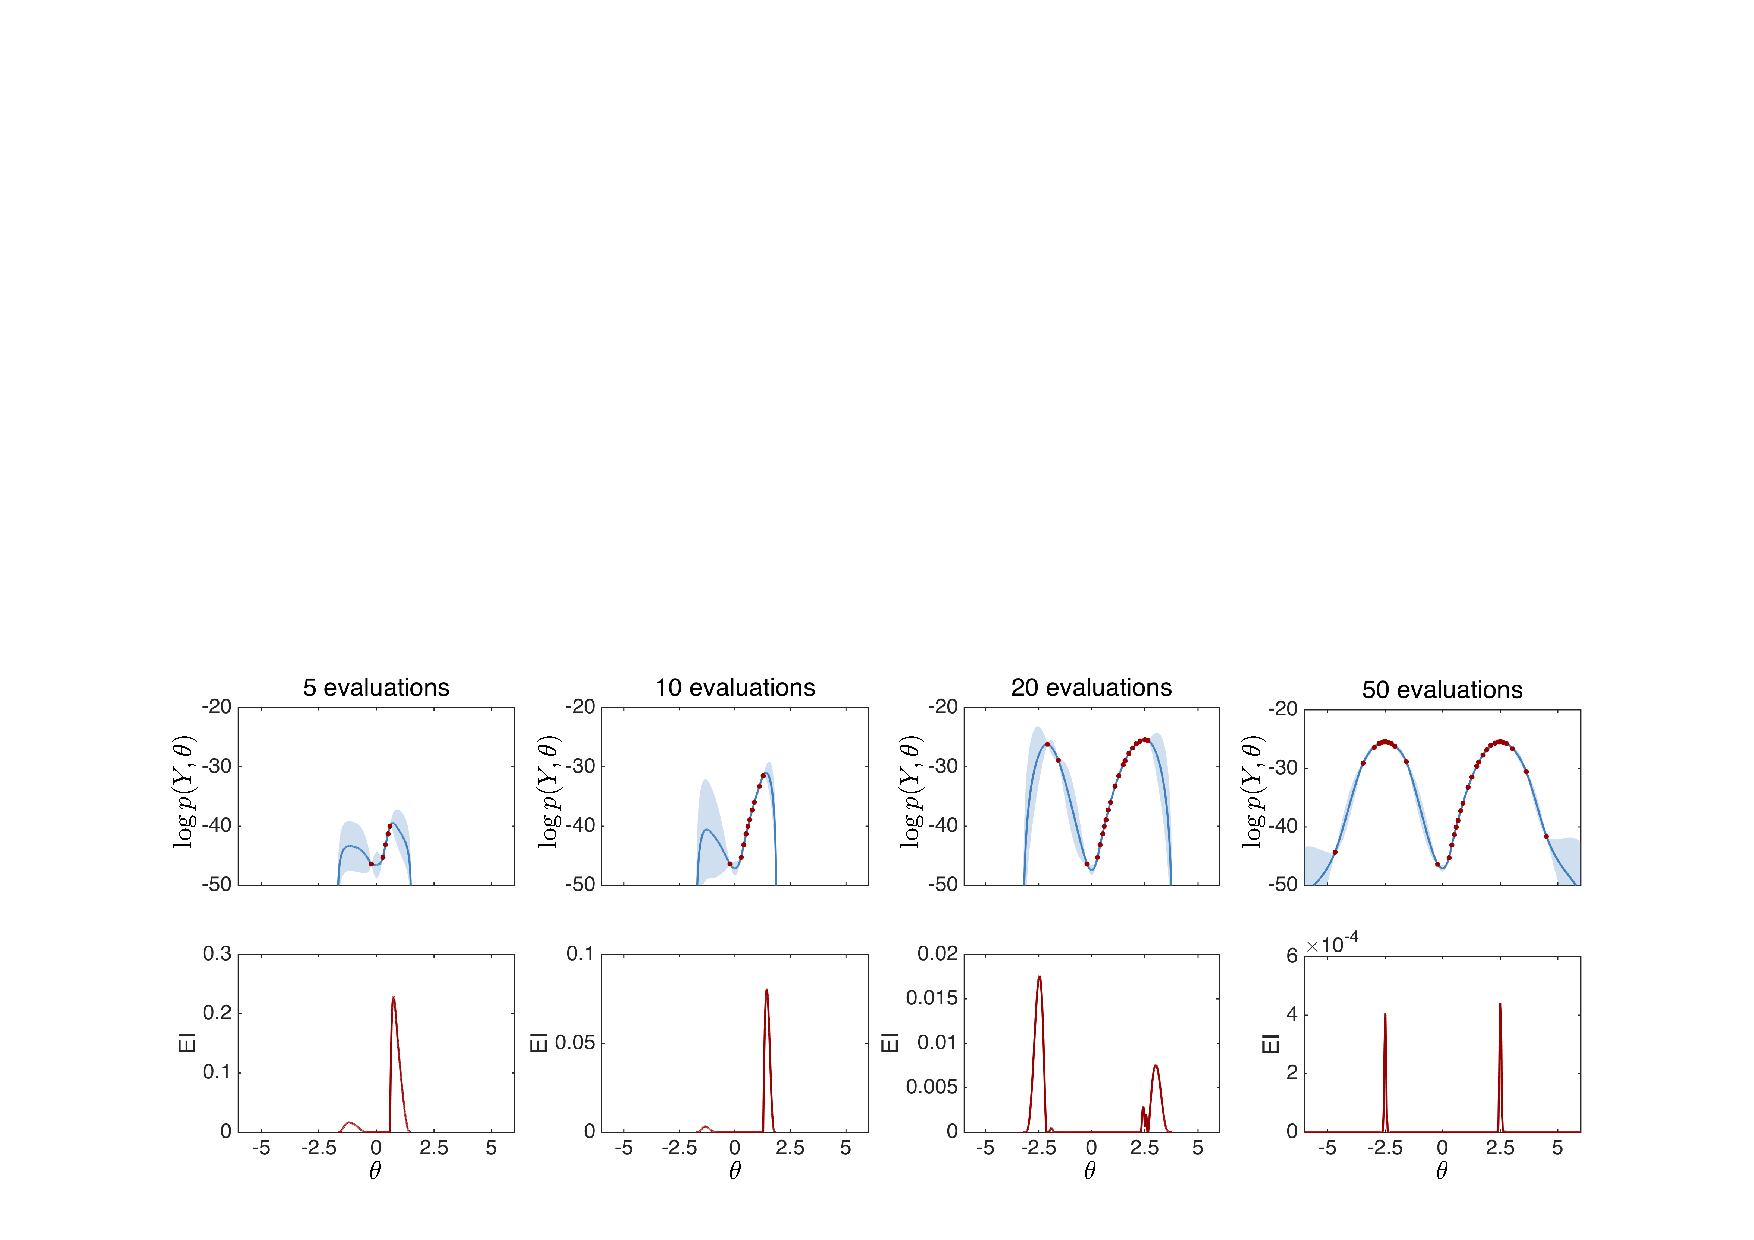
\includegraphics[width=0.99\textwidth]{unbounded_opt}
	\caption{Convergence on an unconstrained bimodal problem with $p \left(\theta\right)={\rm Normal}(0, 0.5)$ and $p \left(Y|\theta\right)={\rm Normal}(5-\left|\theta\right|,0.5)$ giving significant prior misspecification. The top plots show a regressed GP, with the solid line corresponding to the mean and the shading shows $\pm$ 2 standard deviations.  The bottom plots show the corresponding acquisition functions. \label{fig:domainAdpat}}
\end{figure*}

We first demonstrate the ability of BOPP to carry out unbounded optimization using a 1D problem with a significant prior-posterior mismatch as shown in Figure \ref{fig:domainAdpat}.  It shows BOPP adapting to the target and effectively establishing a maxima in the presence of multiple modes.   After 20 evaluations the acquisitions begin to explore the right mode, after 50 both modes have been fully uncovered.

\begin{figure*}[t]
	\centering
	
\includegraphics[width=1\textwidth]{combined_opt_plots}
	%	\includegraphics[width=1.35in]{figures/bayes-opt-comp/branin.pdf}
	%	\includegraphics[width=1.35in]{figures/bayes-opt-comp/hartmann.pdf}
	%	\includegraphics[width=1.35in]{figures/bayes-opt-comp/svm.pdf}
	%	\includegraphics[width=1.35in]{figures/bayes-opt-comp/lda.pdf}
	\caption{Comparison of BOPP  used as an optimizer to prominent BO packages on common benchmark problems.  
		%Branin and Hartmann 6D represent are continuous optimizations, whilst SVM on-grid and LDA on-grid are discrete.  
		The dashed lines shows the final mean error of SMAC (red), Spearmint (green) and TPE (black) as quoted by \cite{eggensperger2013towards}. % which also provides further details on the other packages and the benchmark problems.  
		The dark blue line shows the mean error for BOPP averaged over 100 runs, whilst the median and 25/75\% percentiles are shown in cyan. Results for Spearmint on Branin and SMAC on SVM on-grid are omitted because both BOPP and the respective algorithms averaged zero error to the provided number of significant figures in \cite{eggensperger2013towards}.
		%, meaning it not possible to check where BOPP performed better or worse then the alternative in these two cases.
		\label{fig:bayes-opt}}
\end{figure*}

\subsection{Classic Optimization Benchmarks}

Next we compare BOPP to the prominent BO packages SMAC \cite{hutter2011sequential}, Spearmint \cite{snoek2012practical} and TPE \cite{bergstra2011algorithms} on a number of classical benchmarks as shown in Figure \ref{fig:bayes-opt}.  These results demonstrate that BOPP provides substantial advantages over these systems when used simply as an optimizer on both continuous and discrete optimization problems.  In particular, it offers a large advantage over SMAC and TPE on the continuous problems (Branin and Hartmann), due to using a more powerful surrogate, and over Spearmint on the others due to not needing to make approximations to deal with discrete problems.

\subsection{Marginal Maximum a Posteriori Estimation Problems}

We now demonstrate application of BOPP on a number of MMAP problems.  Comparisons here are more difficult due to the dearth of existing alternatives for PPS.  In particular, simply running inference on the original query does not return estimates for $p\left(Y,\theta\right)$.  We consider the possible alternative of using our conditional code transformation to design a particle marginal Metropolis Hastings (PMMH, \cite{andrieu2010particle}) sampler which operates in a similar fashion to BOPP except that new $\theta$ are chosen using a MH step instead of actively sampling with BO.
%\footnote{To carry out MMAP one could further apply an annealing to the PMMH.  We omit this here as the behaviour of such as system would be indistinguishable from the presented results, due to the small number of iterations and very large variations of $p\left(\theta\right)$ for changes in $\theta$.}
For these MH steps we consider both LMH \citep{wingate2011lightweight} with proposals from the prior and the random-walk MH (RMH) variant introduced in Section~\ref{sec:proginf:str:lmh}.

\subsubsection{Hyperparameter Optimization for Gaussian Mixture Model}

% !TEX root =  bopp.tex


\begin{figure}[t]
	\begin{lstlisting}[basicstyle=\footnotesize\ttfamily]
(defopt mvn-mixture [data mu0 kappa psi] [nu alpha]
 (let [[n d] (shape data)
       alpha (sample (uniform-continuous 0.01 100))
       nu (sample (uniform-continuous (- d 1) 100))
       obs-proc0 (mvn-niw mu0 kappa nu psi)]
       (loop [data data
              obs-procs {}
              mix-proc (dirichlet-discrete 
                          (vec (repeat d alpha)))]
	    (let [y (first data)]
	     (if y
	      (let [z (sample (produce comp-proc))
	            obs-proc (get obs-procs z obs-proc0)
	            obs-dist (produce obs-proc)]
	        (observe obs-dist y)
	        (recur (rest data)
	               (assoc obs-procs z (absorb obs-proc y))
	        (absorb mix-proc z)))
	      mix-proc)))))
	\end{lstlisting}
	\caption{
		\label{fig:mvn-code}
		Anglican query for hyperparameter optimization of a Gaussian mixture model, defined in terms of two parameters \lsi{nu} and \lsi{alpha}. A \lsi{mvn-niw} process is used to represent the marginal likelihood of observations under a Gaussian-inverse-Wishart prior, whereas a \lsi{dirichlet-discrete} process models the prior probability of cluster assignments under a Dirichlet-discrete prior. The command \lsi{produce} returns the predictive distribution for the next sample from a process. \lsi{absorb} conditions on the value of the next sample.}
\end{figure}

\begin{figure*}[t]
	%	\includegraphics[width=1.7in]{"../figures/mvn-mixture/opt-nu-alpha-160229-01-10"}
	%	~
	%	\includegraphics[width=1.7in]{"../figures/mvn-mixture/opt-nu-alpha-160229-01-20"}
	%	~
	%	\includegraphics[width=1.7in]{"../figures/mvn-mixture/opt-nu-alpha-160229-01-50"}
	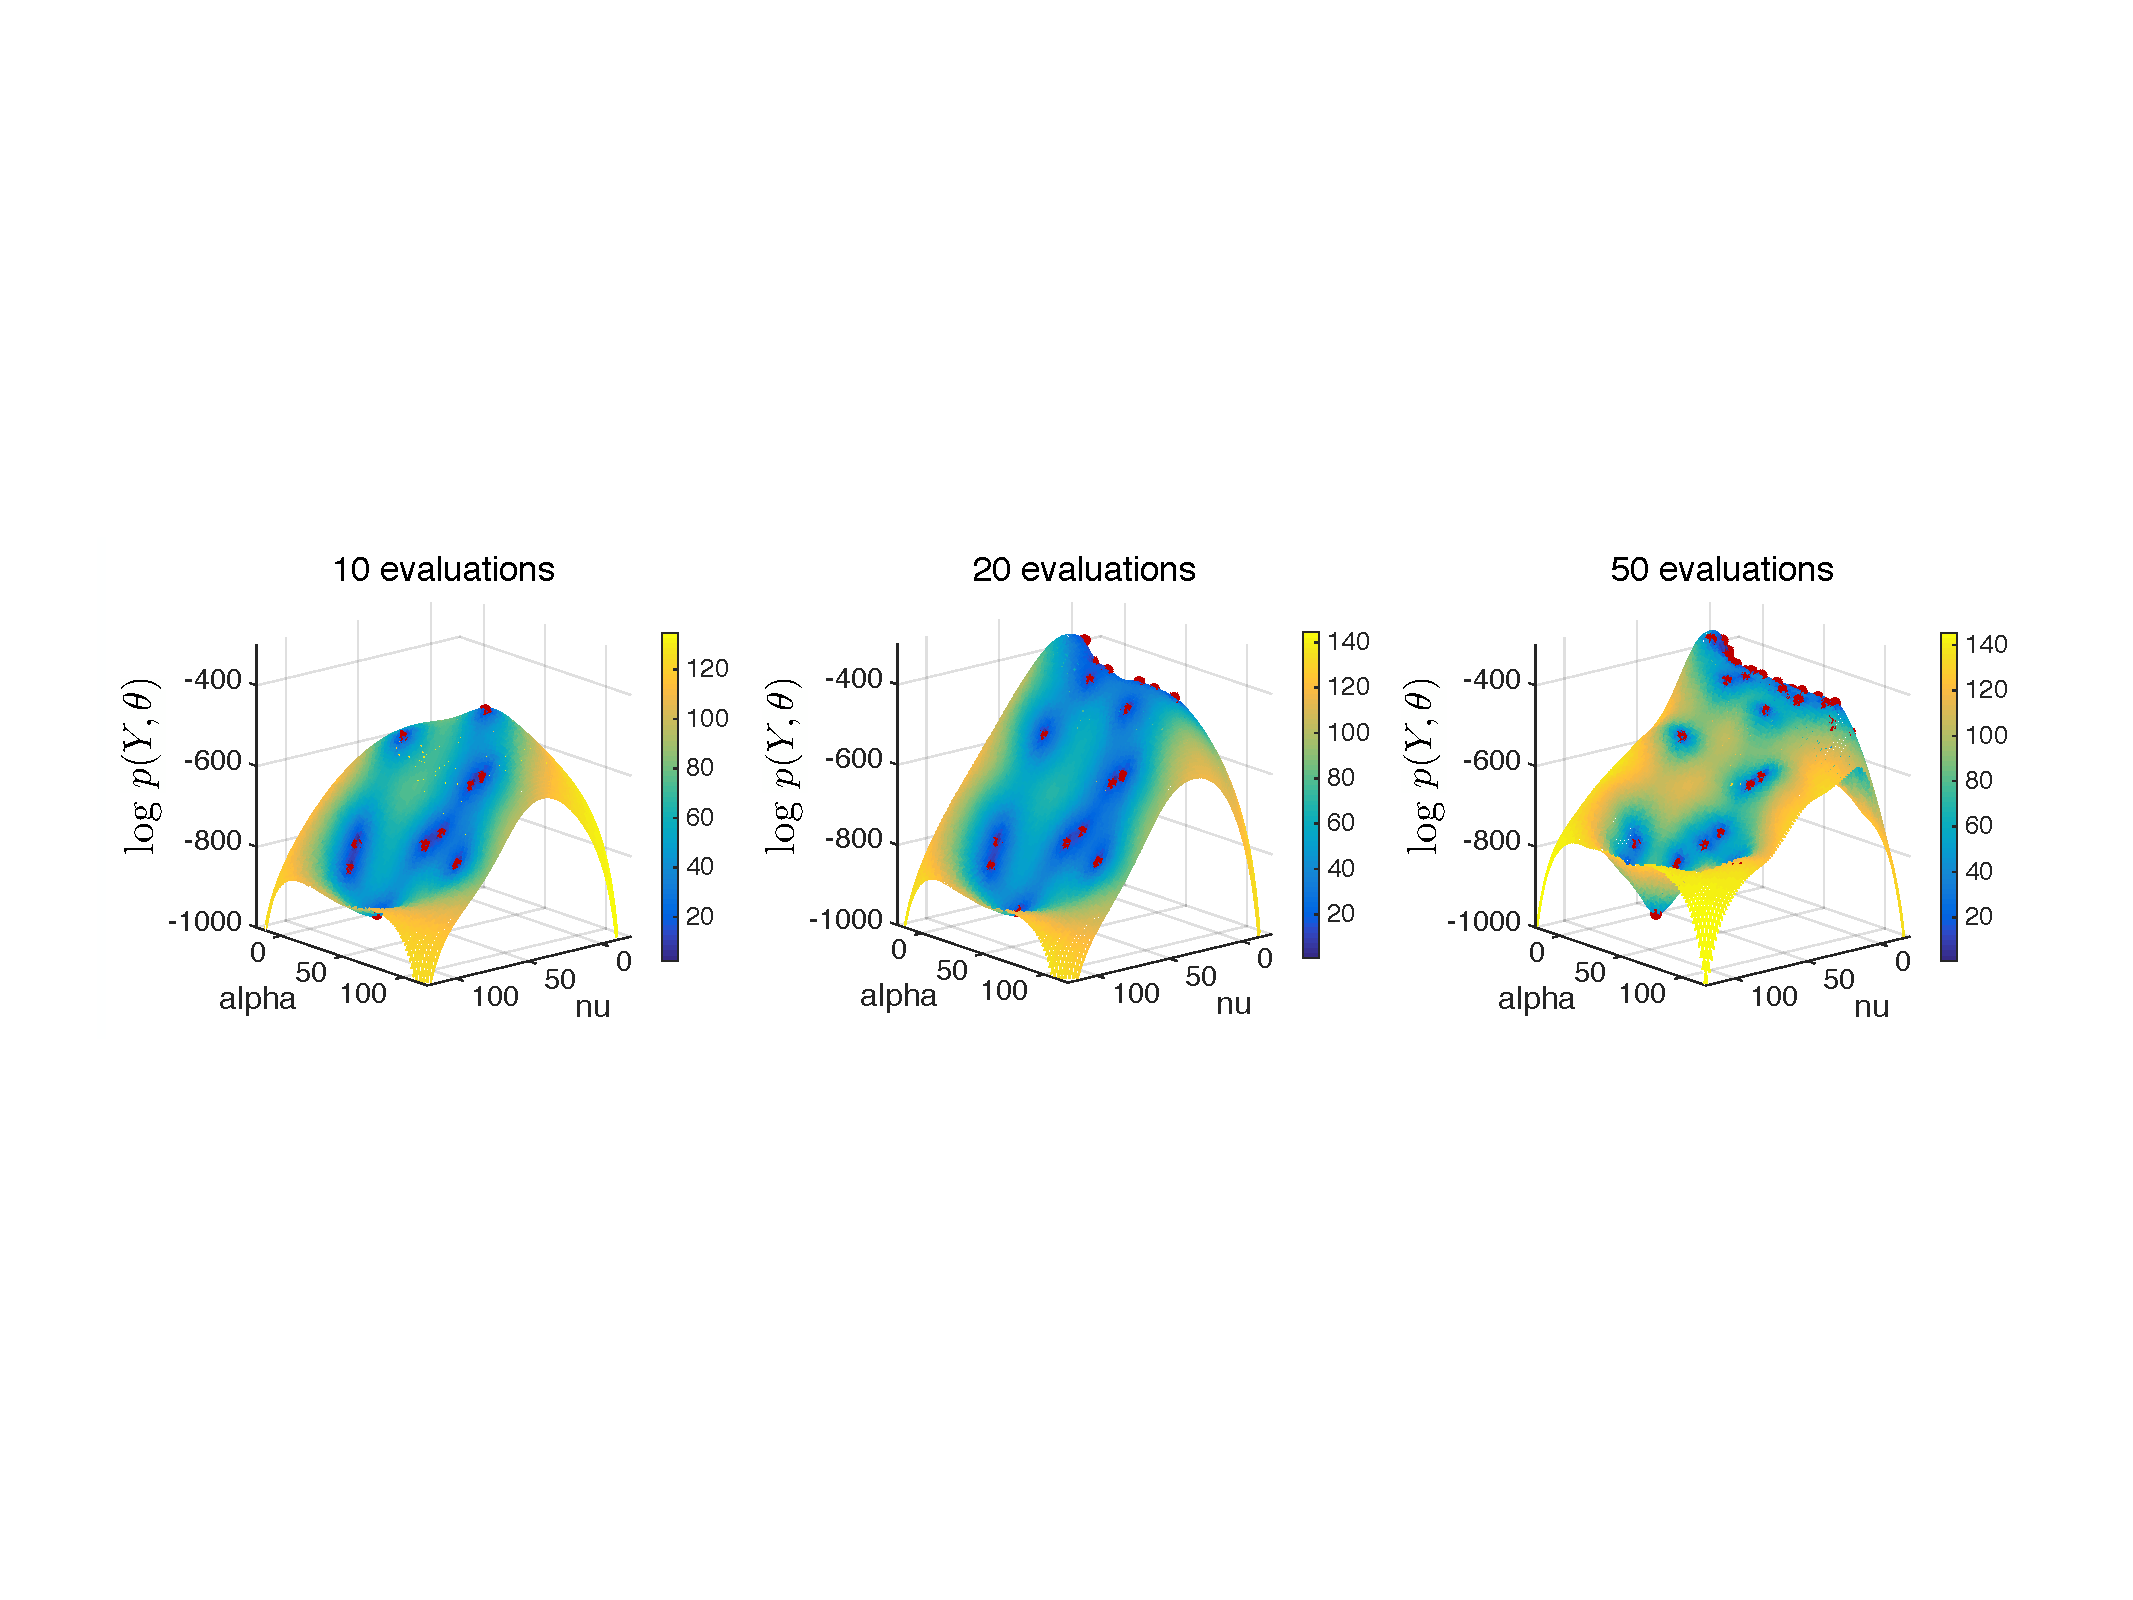
\includegraphics[width=\textwidth]{mvn-mixture/axis_corr_mvn_gps}
	\caption{
		\label{fig:mvn-gp-surface}
		Bayesian optimization of hyperparameters in a Gaussian mixture model evaluated on the Iris dataset. Panels show the GP posterior as a function of number of evaluations, with the surface corresponding to the posterior mean and the color bars the posterior standard deviation. Optimization is performed over the parameter $\alpha$ of a 10-dimensional symmetric Dirichlet distribution and the degrees of freedom $\nu$ of the inverse-Wishart prior. At each evaluation we obtain an estimate of the log marginal $\log p(Y,\theta)$ obtained by performing sequential Monte Carlo inference with 1000 particles.  The apparent maximum after initialization with 10 randomly sampled points lies at $\nu=31$, $\alpha=60$, and $\log p(Y,\theta) = -456.3$ (\emph{left}).  The surface after 10 optimization steps shows a new maximum at $\nu=9.2$, $\alpha=0.8$, and $\log p(Y,\theta) = -364.2$ (\emph{middle}). After 40 steps and 50 total evaluations this optimum is refined to $\nu=16$, $\alpha = 0.2$, and $\log p(Y,\theta) = -352.5$  (\emph{right}).}
\end{figure*}

We start with an illustrative case study of optimizing the hyperparameters in a multivariate Gaussian mixture model. We consider a Bayesian formulation with a symmetric Dirichlet prior on the mixture weights and a Gaussian-inverse-Wishart prior on the likelihood parameters:
\begin{align}
\v{\pi}
&\sim 
{\rm Dir(\alpha, \ldots, \alpha)}
\displaybreak[0]\\
(\v{\mu}_k, \v{\Sigma}_k)
&\sim 
{\rm NIW} (\v{\mu}_0, \kappa, \v{\Psi}, \nu)
&
{\rm for~}
&
k = 1, \ldots , K
\displaybreak[0]\\
z_n 
&\sim 
{\rm Disc(\v{\pi})}
\displaybreak[0]\\
\v{y}_n
&
\sim
{\rm Norm}(\v{\mu}_{z_n}, \v{\Sigma}_{z_n})
&
{\rm for~}
&
n = 1, \ldots , N
\end{align}
% Figure~\ref{fig:mvn-code} shows an optimization query for an Anglican program corresponding to this model. 
Anglican code for this model is shown in Figure 4. Anglican provides stateful objects, which are referred to as random processes, to represent the predictive distributions for the cluster assignments $z$ and the observations $\v{y}^k$ assigned to each cluster
\begin{align}
z_{n+1}
& \sim 
p( \cdot \,|\, z_{1:n}, \alpha),
\\
\v{y}_{m+1}^{k} 
& \sim 
p(\cdot \,|\, \v{y}^k_{1:m}, \v{\mu}_0, \kappa, \v{\Psi}, \nu).
\end{align}
In this collapsed representation marginalization over the model parameters $\v{\pi}$, $\v{\mu}_{k=1:K}$, and $\v{\Sigma}_{k=1:K}$ is performed analytically.
%The only variables that are sampled during program execution are the cluster assignments $z_{1:N}$, which we marginalize over using the general-purpose sequential Monte Carlo (SMC) implementation provided by the inference back end. 
%Like any importance sampling method, SMC provides an unbiased estimate $\hat Z$ of the marginal likelihood $Z = p(\v{y}_{1:N} | \alpha, \v{\mu}, \kappa, \v{\Psi}, \nu)$. 
%Intuitively, the parameter $\nu$, which is known as the degrees of freedom, represents a scale factor for the covariance matrix, which determines the spatial extent of the clusters (larger $\nu$ values imply a smaller covariance and cluster size). 
%The parameter $\alpha$, sometimes known as a concentration parameter, controls the distribution on mixture weights (where $\alpha \gg 1.0$ implies an even distribution and $\alpha \ll 1.0$ implies an uneven distribution).  
Using the Iris dataset, a standard benchmark for mixture models that contains 150 labeled examples with 4 real-valued features, we optimize the marginal with respect to the subset of the parameters $\nu$ and $\alpha$ under uniform priors over a fixed interval.  For this model, BOPP aims to maximize
\begin{align}
\begin{split}
& p(\nu, \alpha | \v{y}_{n=1:N}, \v{\mu}_0, \kappa, \v{\Psi}) \\
&= \iiiint p(\nu, \alpha, z_{n=1:N}, \v{\pi}, \v{\mu}_{k=1:K}, \v{\Sigma}_{k=1:K} | \v{y}_{n=1:N}, \mu_0, \kappa, \v{\Psi}) \mathrm{d}z_{n=1:N}\mathrm{d}\v{\pi}\mathrm{d}\v{\mu}_{k=1:K}\mathrm{d}\v{\Sigma}_{k=1:K}.
\end{split}
\end{align}

Figure~\ref{fig:mvn-gp-surface} shows GP regressions on the evidence after different numbers of the SMC evaluations have been performed on the model.  This demonstrates how the GP surrogate used by BO builds up a model of the target, used to both estimate the expected value of $\log p(Y,\theta)$ for a particular $\theta$ and actively sample the $\theta$ at which to undertake inference.

% n=10
% x1_max: 30.90
% x2_max: 61.55
% y_max: -456.32
% mu_max: -456.33
% sig_max: 0.51

% n=20
% x1_max: 9.20
% x2_max: 0.79
% y_max: -364.21
% mu_max: -364.23
% sig_max: 0.47

% n=50
% x1_max: 16.34
% x2_max: 0.21
% y_max: -352.51
% mu_max: -352.51
% sig_max: 0.53

% n=100
% x1_max: 16.34
% x2_max: 0.21
% y_max: -352.51
% mu_max: -352.50
% sig_max: 0.41

% \begin{figure}
% \begin{lstlisting}[basicstyle=\footnotesize\ttfamily]
% (defopt mvn-mixture 
%  [data mu kappa psi] [:nu :alpha]
%  (let [[n d] (shape data)
%        alpha (sample :alpha
%               (uniform-continuous 0.01 100))
%        nu (sample :nu 
%            (uniform-continuous (- d 1) 100))
%        obs-proc0 (mvn-niw mu kappa nu psi)]
%   (loop [data data
%          obs-procs {}
%          mix-proc (dirichlet-discrete 
%                    (vec (repeat d alpha)))]
%    (let [y (first data)]
%     (if y
%      (let [z (sample (produce comp-proc))
%            obs-proc (get obs-procs 
%                      z obs-proc0)
%            obs-dist (produce obs-proc)]
%       (observe obs-dist y)
%       (recur (rest data)
%              (assoc obs-procs
%                z (absorb obs-proc y))
%              (absorb mix-proc z)))
%      (predict mix-proc))))))
% \end{lstlisting}
% \caption{
% \label{fig:mvn-code}
% Anglican query for hyperparameter optimization of a Gaussian mixture model, defined in terms of two parameters \lsi{:nu} and \lsi{:alpha}. A \lsi{mvn-niw} process is used to represent the marginal likelihood of observations under a Gaussian-inverse-Wishart prior, whereas a \lsi{dirichlet-discrete} process models the prior probability of cluster assignments under a Dirichlet-discrete prior. The command \lsi{produce} returns the predictive distribution for the next sample from a process. \lsi{absorb} conditions on the value of the next sample.}
% \end{figure}





% 


\subsubsection{Extended Kalman Filter for the Pickover Chaotic Attractor}
\label{sec:AppKalman}

% !TEX root =  ../main.tex


\begin{figure*}[t]
	\centering
	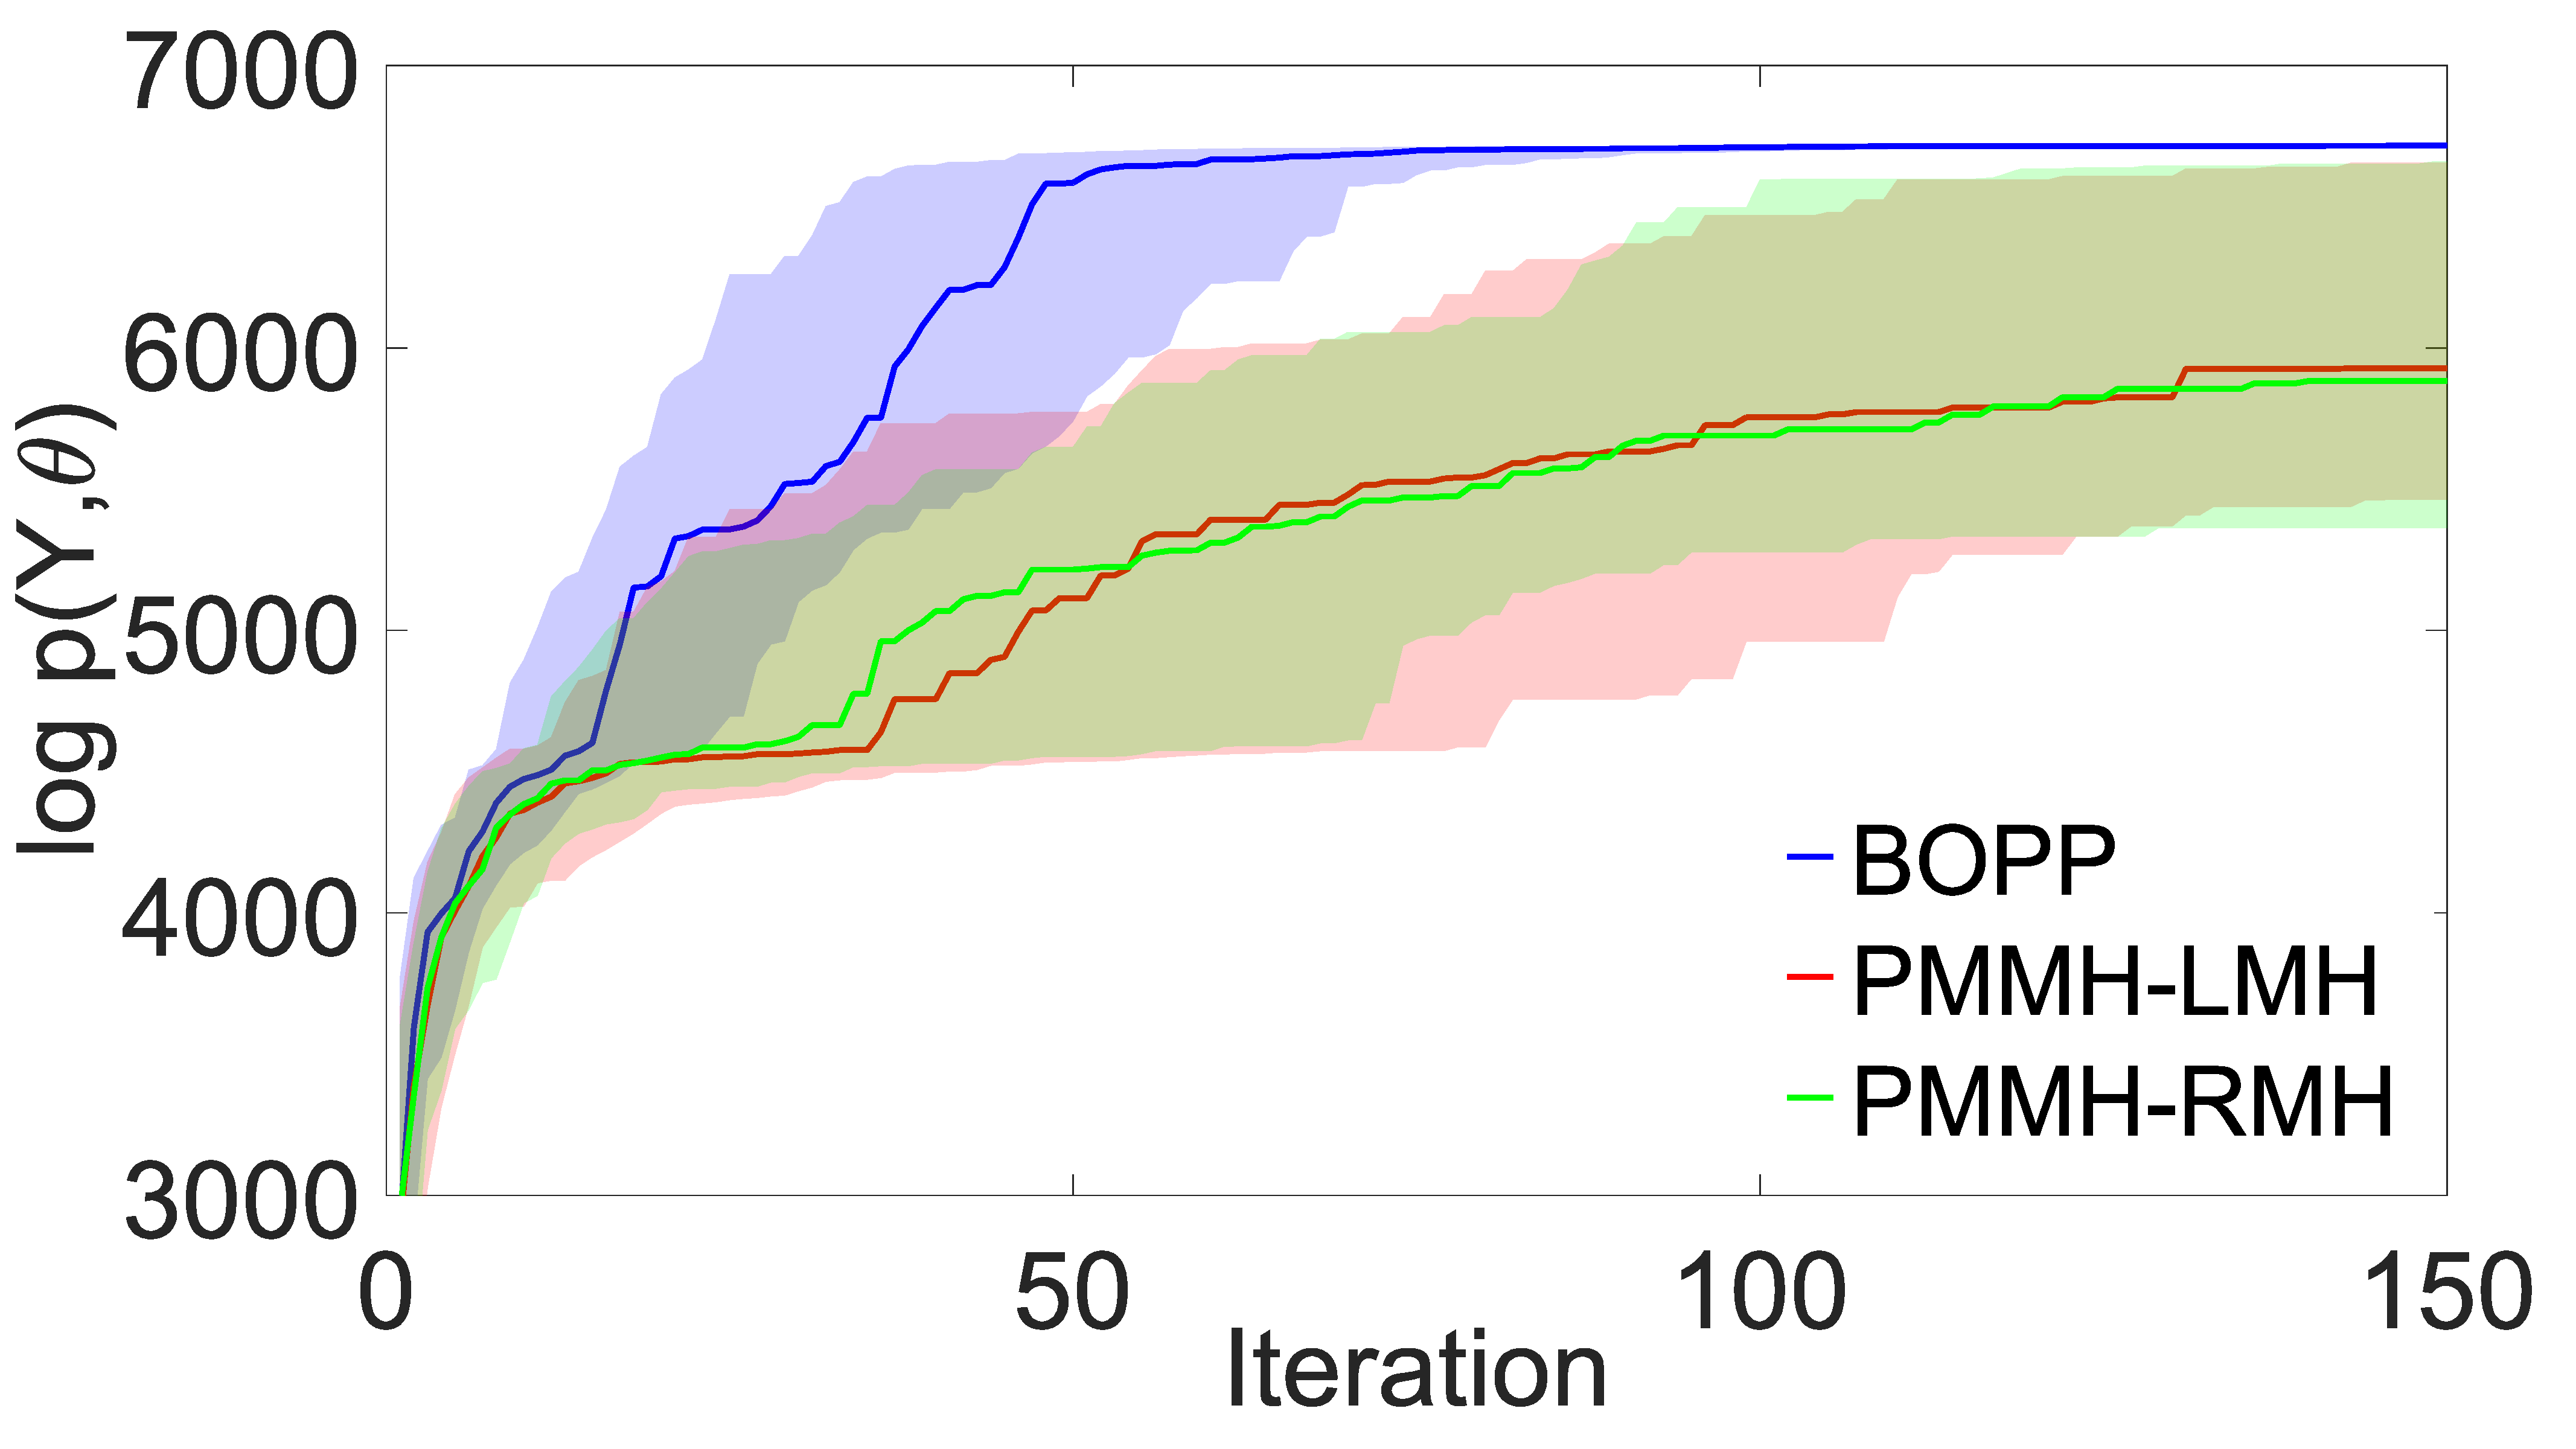
\includegraphics[width=2.72in]{chaos/chaos_ml.pdf}
	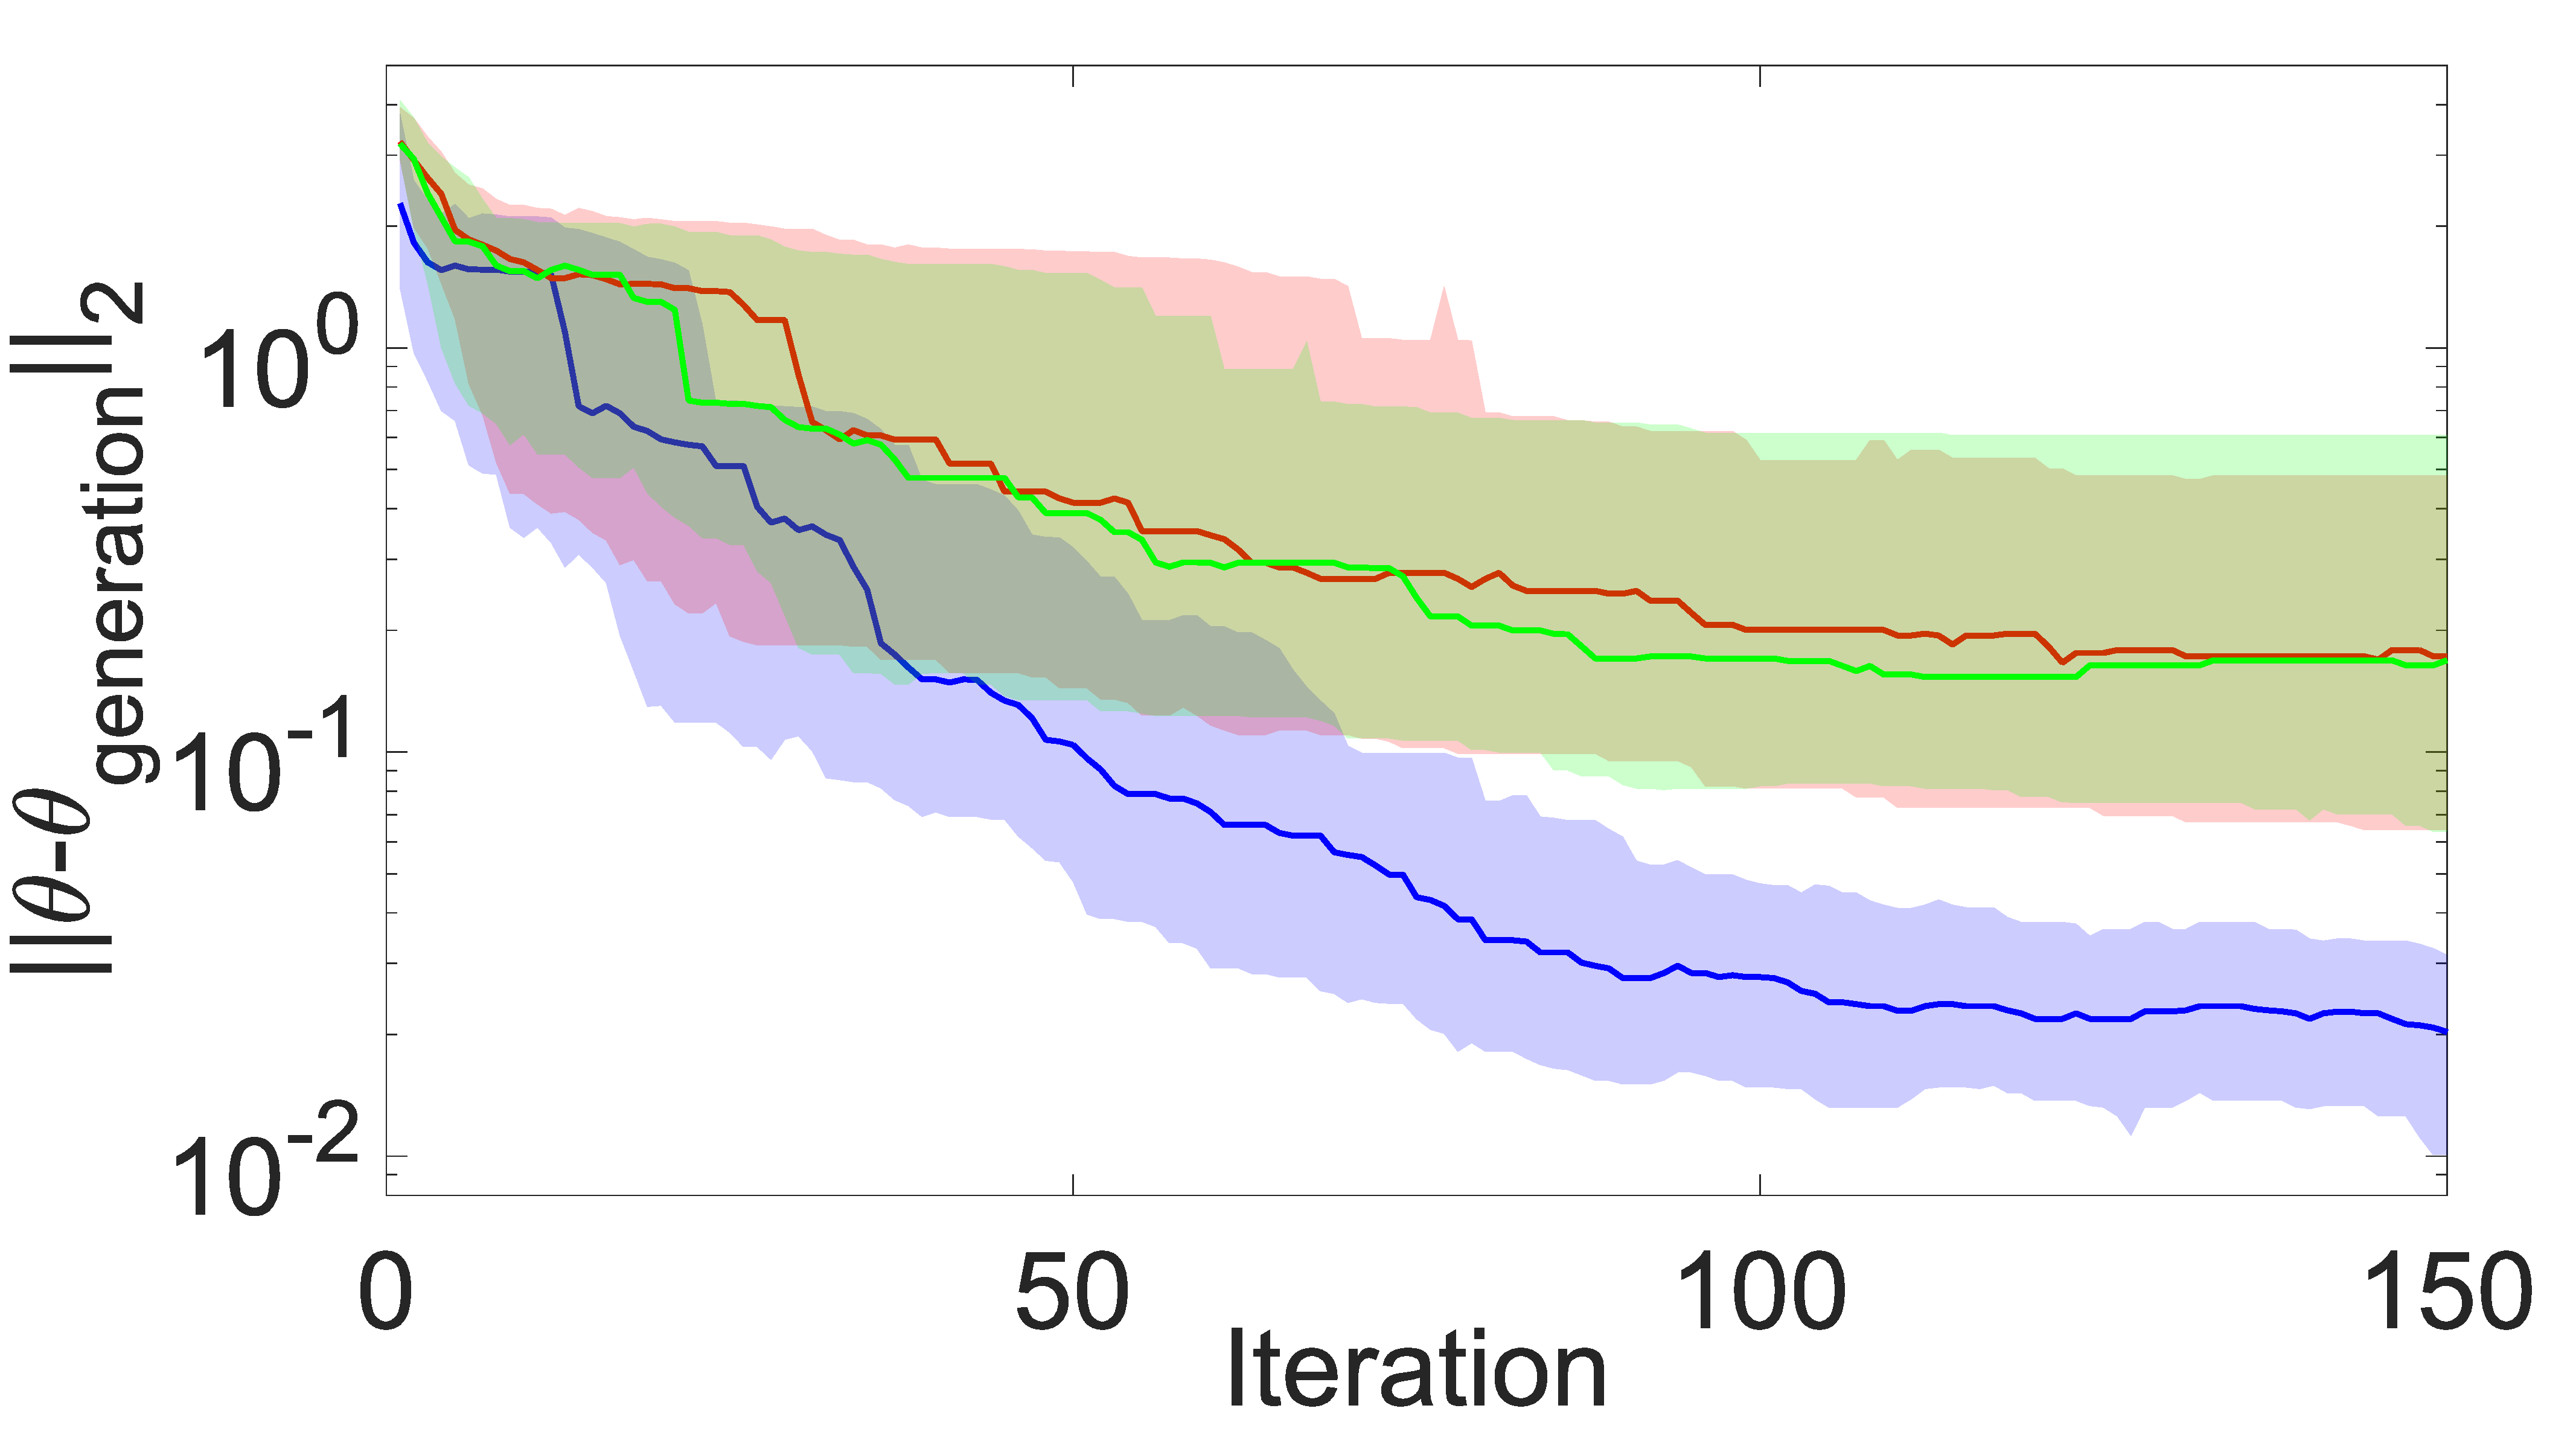
\includegraphics[width=2.72in]{chaos/chaos_distance.pdf}
	\caption{Convergence for transition dynamics parameters of the pickover attractor in terms of the cumulative best $\log p\left(Y,\theta\right)$ (\emph{left}) and distance to the ``true" $\theta$ used in generating the data (\emph{right}). Solid line shows median over 100 runs, whilst the shaded region the 25/75\% quantiles.  \label{fig:chaos}
		\vspace{6pt}}
\end{figure*}

\begin{figure}[t]
	\centering
	\begin{subfigure}[t]{0.24\textwidth}
		\centering
		
\includegraphics[height=3.2cm,width=3.7cm]{chaos/compressed/first_iter_alt.png}
		\caption{1 iteration}
	\end{subfigure}
	\begin{subfigure}[t]{0.24\textwidth}
		\centering
		\tiny
		
\includegraphics[height=3.2cm,width=3.7cm]{chaos/compressed/20_iter_alt.png}
		\caption{20 iterations}
	\end{subfigure}
	\begin{subfigure}[t]{0.24\textwidth}
		\centering
		\tiny
		
\includegraphics[height=3.2cm,width=3.7cm]{chaos/compressed/100_iter_altj.png}
		\caption{100 iterations}
	\end{subfigure}
	\begin{subfigure}[t]{0.24\textwidth}
		\centering
		\tiny
		
\includegraphics[height=3.2cm,width=3.7cm]{chaos/compressed/target_light.png}
		\caption{Ground truth}
	\end{subfigure}
	\caption{A series of trajectories for different parameters, demonstrating convergence to the true attractor.  The colormap is based on the speed and curvature of the trajectory, with rendering done using the program Chaoscope (available at {\href{http://www.chaoscope.org/}{http://www.chaoscope.org/}}). \label{fig:chaoscope}}
\end{figure}

Our first MMAP example considers the case of learning the dynamics parameters of a chaotic attractor.  
This constitutes a class Markovian state space model problem, specifically a Kalman smoother,
where we observe a noisy signal 
$y_t \in \real^{K}, \; t = 1,2,\dots,T$ in some $K$ dimensional observation space were each 
observation has a lower dimensional latent parameter $x_t \in \real^{D},  \; t = 1,2,\dots,T$.
In addition to an initial distribution $x_1 \sim \mathcal{N} \left(\mu_1, \sigma_1 I\right)$, our model is specified by 
\begin{subequations}
	\label{eq:Kalman}
\begin{align}
x_t = & A \left(x_{t-1}, \theta\right)+\delta_{t-1}, \; & \delta_{t-1} \sim \mathcal{N} \left(0, \sigma_q I\right) \\
y_t = & C x_{t}+\varepsilon_{t}, \; & \varepsilon_{t} \sim \mathcal{N} \left(0, \sigma_y I\right)
\end{align}
\end{subequations}
where $I$ is the identity matrix, $C$ is a known $K \times D$ matrix, and $\mu_1,\sigma_1, \sigma_q$ 
and $\sigma_y$ are all known scalars.  Our aim is to learn the dynamics parameters $\theta$ given
$y_{1:T}$, marginalizing over the latent variables $x_{1:T}$.  We use
a uniform prior on the parameters $\theta$, which means that the MMAP values for $\theta$
coincide with their (constrained) MML values.  A synthetic dataset was generated with $T=500$ and
$K=20$ (see \cite{rainforth2017boppArxiv}).
Inference on \qmarg was carried out using SMC with 500 particles.  
Convergence results are given in Figure~\ref{fig:chaos} showing that BOPP comfortably 
outperforms the PMMH variants, while Figure~\ref{fig:chaoscope} shows the simulated 
attractors generated from the dynamics parameters output by various iterations of a 
particular run of BOPP.


\subsubsection{Hidden Markov Model with Unknown Number of States}

% !TEX root =  ../main.tex

\begin{figure*}[t]
	\centering
	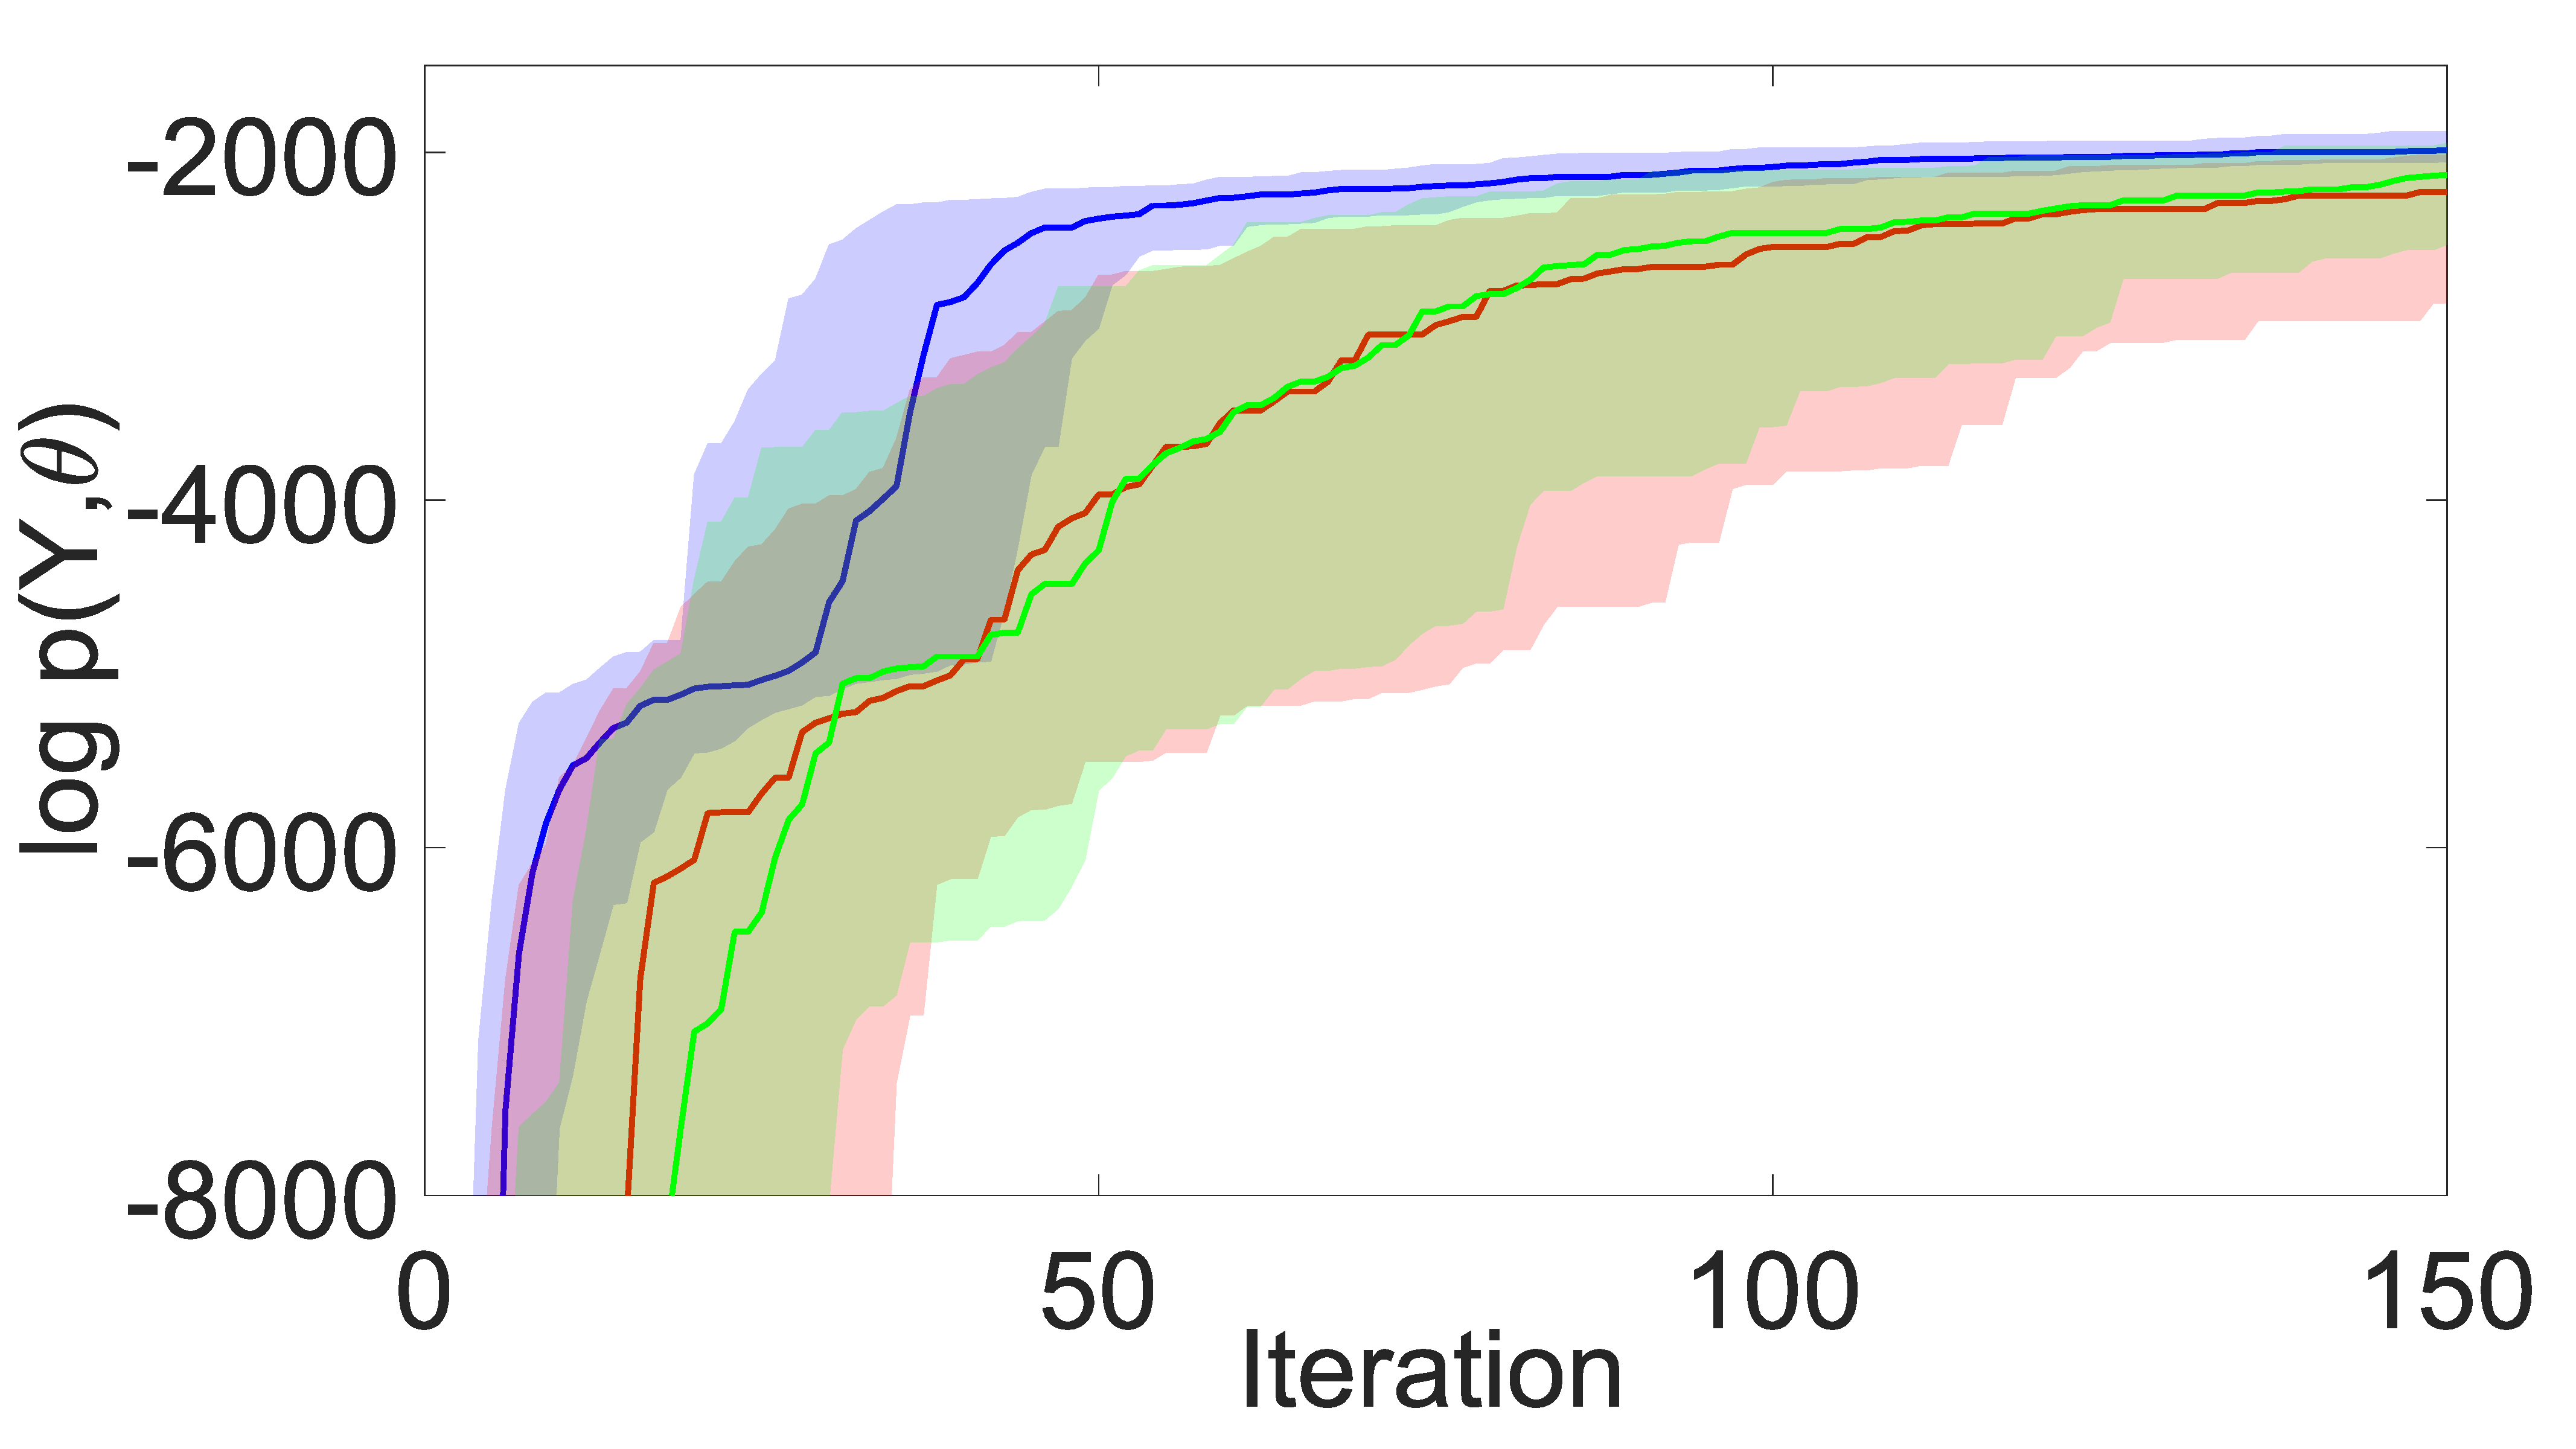
\includegraphics[width=2.72in]{hmm/hmm_ML}
	~~~~~~
	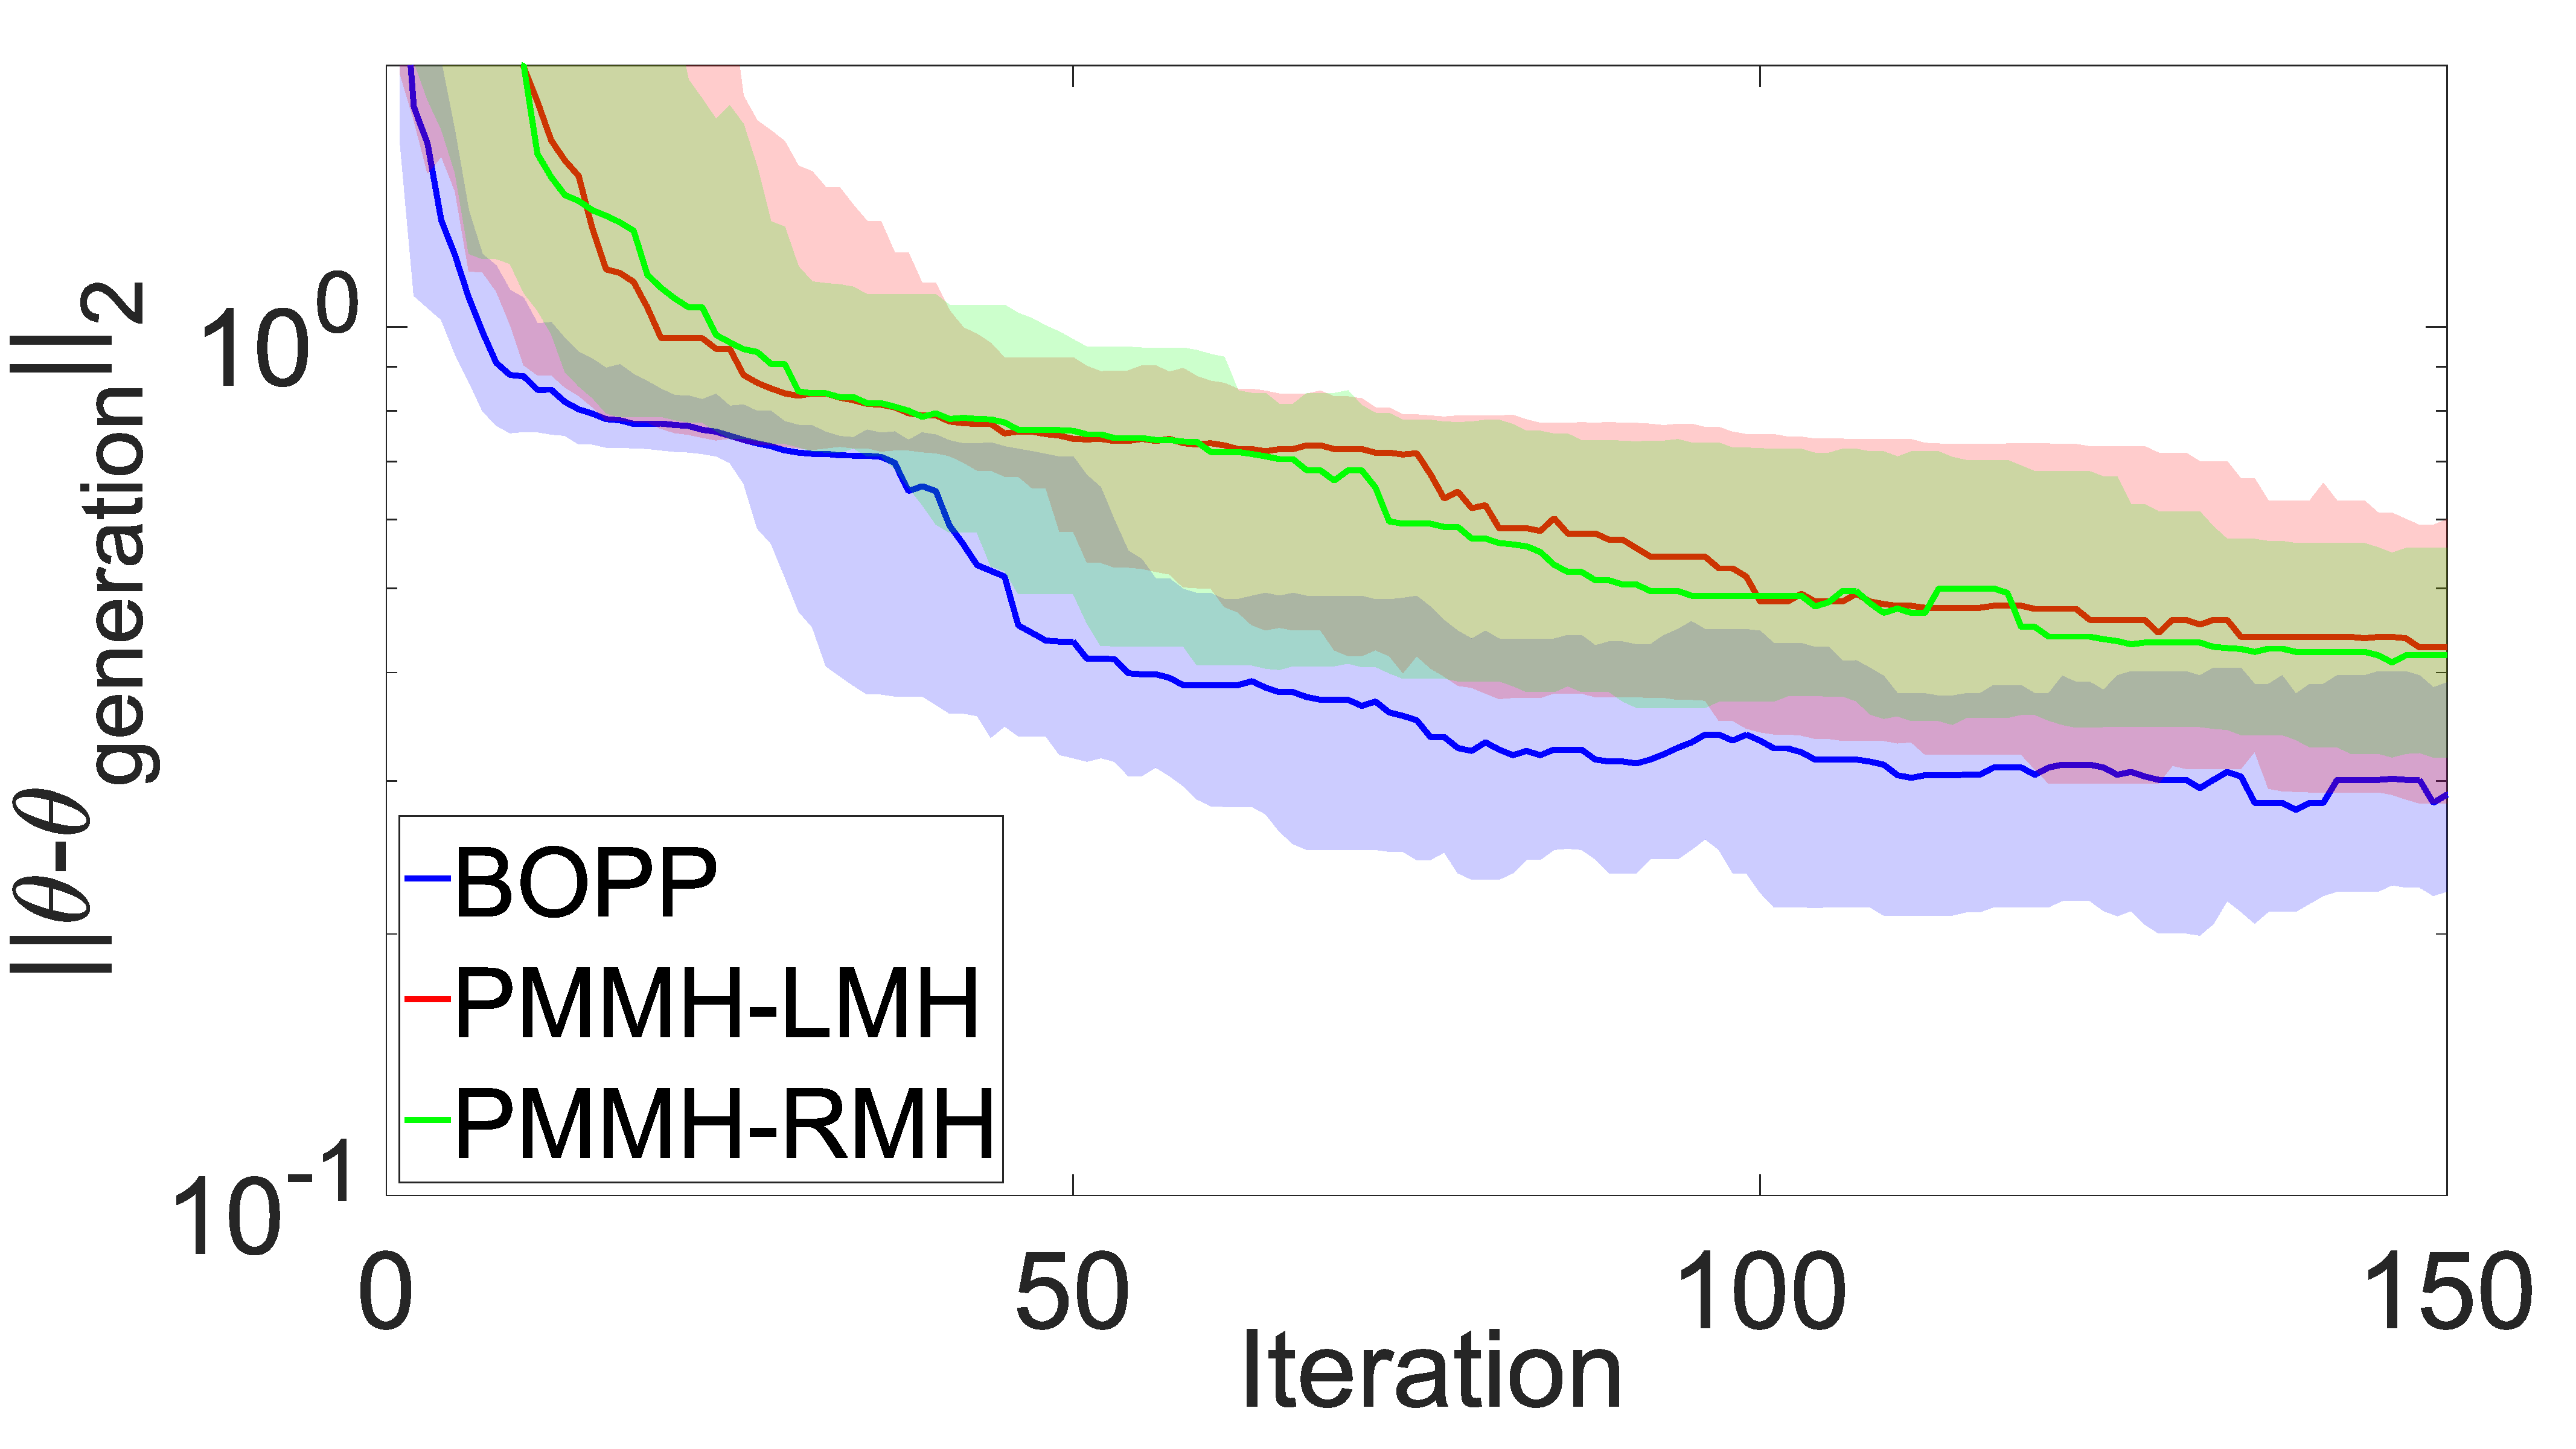
\includegraphics[width=2.72in]{hmm/hmm_distance}
	\caption{Convergence for HMM in terms of the cumulative best $\log p\left(Y,\theta\right)$ (\emph{left}) and distance to the ``true" $\theta$ used in generating the data (\emph{right}). Solid line shows median over 100 runs, whilst the shaded region the 25/75\% quantiles.  Note that for the distance to true $\theta$ was calculated by selecting the three states (out of the 5 generated) that were closest to the true parameters.  \label{fig:hmm}}
\end{figure*}

We finish by considering a hidden Markov model (HMM) with an unknown number of discrete possible states.  
This example demonstrates how BOPP can still be applied to models which conceptually have an 
unknown number of target variables, by generating all possible variables that might be needed, 
but then leaving some variables unused for some execution traces.  This avoids problems 
of varying reference measures so that the MMAP problem is well defined  and provides a 
function with a fixed number of inputs as required by the BO scheme.  From the BO 
perspective, the target function is simply constant for variations in an unused variable.

Our model places a uniform prior on the number of states $K \sim \textsc{Discrete}\{1,2,3,4,5\}$.
Each emission distribution corresponds to a Gaussian with unknown mean (which we wish to
optimize) and known variance.  
We marginalize over are the transition distribution parameters and the HMM latent states.  
Rather than constructing a model were the emission distribution
parameters only exist conditioned on the value of $K$, we generate variables for all $5$ emission
distributions that might be required, with only the first $K$ actually then used.  
A synthetic dataset was generated using $K=3$ and $T=1000$ observations.  Results of running BOPP are given
in Figure~\ref{fig:hmm}, again showing that BOPP outperforms these PMMH alternatives.  See~\cite{rainforth2017boppArxiv}
for further details.


%
%\subsection{Full Details for House Heating Experiment}
%\label{sec:app:heating}
%
%% !TEX root =  bopp.tex

In this case study, illustrated in Figure~\ref{fig:houses}, we optimize the parameters of a stochastic engineering simulation. We use the Energy2D system from \cite{xie2012energy2d} to perform finite-difference numerical simulation of the heat equation and Navier-Stokes equations in a user-defined geometry. 

In our setup, we designed a 2-dimensional representation of a house with 4 interconnected rooms using the GUI provided by Energy2D. The left side of the house receives morning sun, modelled at a constant incident angle of $30^\circ$. We assume a randomly distributed solar intensity and simulate the heating of a cold house in the morning by 4 radiators, one in each of the rooms. The radiators are given a fixed budget of total power density $P_{\text{budget}}$. The optimization problem is to distribute this power budget across radiators in a manner that minimizes the variance in temperatures across 8 locations in the house. 

Energy2D is written in Java, which allows the simulation to be integrated directly into an Anglican program that defines a prior on model parameters and an ABC likelihood for evaluating the utility of the simulation outputs. Figure \ref{fig:house-heating-code} shows the corresponding program query. In this, we define a Clojure function \lsi{simulate} that accepts a solar power intensity $I_{\text{sun}}$ and power densities for the radiators $P_{\text{r}}$, returning the thermometer temperature readings $\{T_{i, t}\}$. We place a symmetric Dirichlet prior on $\frac{P_r}{P_{\text{budget}}}$ and a gamma prior on $\frac{I_{\text{sun}}}{I_{base}}$, where $P_{\text{budget}}$ and $I_{base}$ are constants. This gives the generative model:
 \begin{align}
 p_r &\sim \Dirichlet([1,1,1,1]) \\
 P_r &\leftarrow P_{\text{budget}} \cdot p_r \\
 \upsilon &\sim \text{Gamma}(5,1) \\
 I_{\text{sun}} &\leftarrow I_{\text{base}} \cdot \upsilon.
 \end{align}
After using these to call \lsi{simulate}, the standard deviations of the returned temperatures is calculated for each time point,
\begin{align}
\omega_t = \sqrt{\sum_{i=1}^8 T_{i, t}^2 -\left(\sum_{i=1}^8 T_{i, t}\right)^2}
\end{align}
and used in the ABC likelihood \lsi{abc-likelihood} to weight the execution trace using a multivariate Gaussian:
\begin{align*}
p\left(\{T_{i, t}\}_{i = 1:8, t = 1:\tau}\right) = \text{Normal}\left(\omega_{t=1:\tau};\mathbf{0},\sigma_T^{2}\mathbf{I}\right)
\end{align*}
where $\mathbf{I}$ is the identity matrix and $\sigma_T = 0.8 ^{\circ} \mathrm{C}$ is the observation standard deviation.

Figure \ref{fig:houses} demonstrates the improvement in homogeneity of temperatures as a function of total number of simulation evaluations. Visual inspection of the heat distributions also shown in Figure \ref{fig:houses} confirms this result, which serves as an exemplar of how BOPP can be used to estimate marginally optimal simulation parameters.


\section{Discussion and Future Work}
\label{sec:disc}

% !TEX root =  bopp.tex

We have introduced a new method for carrying out MMAP estimation of probabilistic program variables using Bayesian optimization, representing the first unified framework for optimization and inference of probabilistic programs.  By using a series of code transformations, our method allows an arbitrary program to be optimized with respect to a defined subset of its variables, whilst marginalizing out the rest.  To carry out the required optimization, we introduce a new GP-based BO package that exploits the availability of the target source code to provide a number of novel features, such as automatic domain scaling and constraint satisfaction.  

The concepts we introduce lead directly to a number of extensions of interest, including but not restricted to smart initialization of inference algorithms, adaptive proposals, and nested optimization.  Further work might consider maximum marginal likelihood estimation and risk minimization.  Though only requiring minor algorithmic changes, these cases require distinct theoretical considerations.
%Another interesting possible extension would be to to apply Bayesian quadrature \cite{osborne2012active} to probabilistic programs.

%Although our implementation is currently restricted to optimize numerical variables of fixed dimensionality, it is possible to extend to a more general case using appropriate kernels, such as the arc kernels introduced by \cite{swersky2014raiders}, which cater to scenarios where certain variables may only exist conditioned on the values of other variables.

%\section{Program Transformations in Detail}
%\label{sec:program-transformations}
%% !TEX root = ../main.tex

In this section we give a more detailed and language specific description of our program transformations, code for which can be found at \href{http://www.github.com/probprog/bopp}{\url{http://www.github.com/probprog/bopp}}. %We will refer to the code in explaining the implementation of program transformations for BOPP.

\subsection{Anglican}
Anglican is a probabilistic programming language integrated into Clojure (a dialect of Lisp) and inherits most of the corresponding syntax. Anglican extends Clojure with the special forms \sample and \observe \citep{tolpin2015probabilistic}.  
Each random draw in an Anglican program corresponds to a \sample  call, which can be thought of as a term in the prior. 
Each \observe statement applies weighting to a program trace and thus constitutes a term in the likelihood.
Compilation of an Anglican program, performed by the macro \lsi{query}, corresponds to transforming the code into a variant of continuation-passing style (CPS) code, which results in a function that can be executed using a particular inference algorithm.

Anglican program code is represented by a nested list of expressions, symbols, non-literals for contructing data structures (e.g. \lsi{[...]} for vectors), and command dependent literals (e.g. \lsi{[...]} as a second argument of a \lsi{let} statement which is used for binding pairs).  In order to perform program transformations, we can recursively traverse this nested list which can be thought of as an abstract syntax tree of the program.

Our program transformations also make use of the Anglican forms \lsi{store} and \lsi{retrieve}.  These allow storing any variable in the probabilistic program's execution trace in a state which is passed around during execution and from which we can retrieve these stored values.  The core use for this is to allow the outer query to return variables which are only locally scoped.

To allow for the early termination that will be introduced in Section \ref{sec:bopp-supp/early-term}, it was necessary to add a mechanism for non-local returns to Anglican.  Clojure supports non-local returns only through Java exception handling, via the keywords {\bf\ttfamily\color{cyan} try}~{\bf\ttfamily\color{cyan}throw},~{\bf\ttfamily\color{cyan}catch} and {\bf\ttfamily\color{cyan}finally}.  Unfortunately, these are not currently supported by Anglican and their behaviour is far from ideal for our purposes.  In particular, for programs containing nested {\bf\ttfamily\color{cyan}try} statements, throwing to a particular {\bf\ttfamily\color{cyan}try} in the stack, as opposed to the most recently invoked, is cumbersome and error prone.
%
%Firstly, return values are stored within exceptions which is cumbersome and can cause issues in debugging.  Secondly, it is difficult to control the point of return.  For example, imagine we wish to return from the query itself and so wrap the original query in a {\bf\ttfamily\color{cyan}try-catch} block.  Na\"{i}vely throwing might now cause us to return to an unexpected point if the original query already contained a {\bf\ttfamily\color{cyan}try-catch} block.  Thus controlling the exact return point would require a careful and error-prone mechanism based on custom exception types and catches.

We have instead, therefore, added to Anglican a non-local return mechanism based on the Common Lisp control form \lsi{catch/throw}.  This uses a \emph{catch tag} to link each \lsi{throw} to a particular \lsi{catch}.  For example
\begin{lstlisting}[basicstyle=\footnotesize\ttfamily]
(catch :tag
  (when (> a 0)
    (throw :tag a))
  0)
\end{lstlisting}
is equivalent to \lsi{(max a 0)}.  More precisely, \lsi{throw} has syntax \lsi{(throw tag value)} and will cause the \lsi{catch} block with the corresponding \lsi{tag} to exit, returning \lsi{value}.   If a \lsi{throw} goes uncaught, i.e. it is not contained within a \lsi{catch} block with a matching tag, a custom Clojure exception is thrown.

%To allow for the early termination discussed in Section \ref{sec:bopp-supp/early-term}, it was necessary to add one new primitive to Anglican, namely \lsi{return} with syntax \lsi{(return return-val)}.  At a high level, \lsi{return} causes the query to terminate, returning \lsi{return-val}.  This is done by, during runtime of the CPS compiled code, returning a Clojure record \lsi{->result} containing \lsi{return-val} instead of a valid program continuation, causing the query execution to terminate and return the required value.

\subsection{Representations in the Main Paper}
\label{sec:bopp-supp/main-paper-rep}

In the main paper we presented the code transformations as static transformations as shown in Figure~\ref{fig:bopp_overview}.  Although for simple programs, such as the given example, these transformations can be easily expressed as static transformations, for more complicated programs it would be difficult to actually implement these as purely static generic transformations in a higher-order language.  Therefore, even though all the transformations dynamically execute as shown at runtime, in truth, the generated source code for the prior and acquisition transformations varies from what is shown and has been presented this way in the interest of exposition.  Our true transformations exploit \lsi{store}, \lsi{retrieve}, \lsi{catch} and \lsi{throw} to generate programs that dynamically execute in the same way at run time as the static examples shown, but whose actual source code varies significantly.

\subsection{Prior Transformation}
\label{sec:bopp-supp/prior-transformations}
The prior transformation recursively traverses the program tree and applies two local transformations.  
Firstly it replaces all \observe statements by \lsi{nil}.  
As \observe statements return \lsi{nil}, this trivially preserves the generative model of the program, but the probability of the execution changes. 
Secondly, it inspects the binding variables of \lsi{let} forms in order to modify the binding expressions for the optimization variables, as specified by the second input of \defopt, asserting that these are directly bound to a \sample statement of the form \texttt{(\sample dist)}.
The transformation then replaces this expression by one that stores the result of this sample in Anglican's \lsi{store} before returning it.
Specifically, if the binding variable in question is \lsi{phi-}$\ell$, then the original binding expression \lsi{(sample dist)} is transformed into
% \begin{figure}
    \begin{lstlisting}[basicstyle=\footnotesize\ttfamily]
(let [value (sample dist)]
  ;; Store the sampled value in Anglican's store
  (store OPTIM-ARGS-KEY
         'phi-$\ell$
         value)
  value)
    \end{lstlisting}
%     \caption{}
%     \label{fig:prior-1}
% \end{figure}

After all these local transformation have been made, we wrap the resulting query block in a \lsi{do} form and append an expression extracting the optimization variables using Anglican's \lsi{retrieve}.  This makes the optimization variables the output of the query.  Denoting the list of optimization variable symbols from \defopt as \lsi{optim-args} and the query body after applying all the above location transformations as \dots, the prior query becomes
% \begin{figure}
    \begin{lstlisting}[basicstyle=\footnotesize\ttfamily]
(query query-args
  (do
    ...
    (map (fn [x] (retrieve OPTIM-ARGS-KEY x))
       optim-args)))
    \end{lstlisting}
%     \caption{}
%     \label{fig:prior-3}
% \end{figure}
Note that the difference in syntax from Figure~\ref{fig:bopp_overview} is because \lsi{defquery} is in truth a syntactic sugar allowing users to bind \lsi{query} to a variable.  As previously stated, \lsi{query} is macro that compiles an Anglican program to its CPS transformation.  An important subtlety here is that the order of the returned samples is dictated by \lsi{optim-args} and is thus independent of the order in which the variables were actually sampled, ensuring consistent inputs for the BO package.

We additionally add a check (not shown) to ensure that all the optimization variables have been added to the store, and thus sampled during the execution, before returning.  This ensures that our assumption that each optimization variable is assigned for each execution trace is satisfied.

\subsection{Acquisition Transformation}
\label{sec:bopp-supp/acq-transformations}
The acquisition transformation is the same as the prior transformation except we append the acquisition function, \lsi{ACQ-F}, to the inputs and then \observe its application to the optimization variables before returning.
The acquisition query is thus
% \begin{figure}
    \begin{lstlisting}[basicstyle=\footnotesize\ttfamily]
(query [query-args ACQ-F]
  (do
    ...
    (let [theta (map (fn [x] (retrieve OPTIM-ARGS-KEY x))
                      optim-args)]
      (observe (factor) (ACQ-F theta))
      theta)))
    \end{lstlisting}
%     \caption{}
%     \label{fig:acq-1}
% \end{figure}

\subsection{Early Termination}
\label{sec:bopp-supp/early-term}
To ensure that \lsi{q-prior} and \lsi{q-acq} are cheap to evaluate and that the latter does not include unnecessary terms which complicate the optimization, we wish to avoid executing code that is not required for generating the optimization variables.
Ideally we would like to directly remove all such redundant code during the transformations.
However, doing so in a generic way applicable to all possible programs in a higher order language represents a significant challenge.
Therefore, we instead transform to programs with additional early termination statements, triggered when all the optimization variables have been sampled.  
Provided one is careful to define the optimization variables as early as possible in the program (in most applications, e.g. hyperparameter optimization, they naturally occur at the start of the program), this is typically sufficient to ensure that the minimum possible code is run in practise.

To carry out this early termination, we first wrap the query in a \lsi{catch} block with a uniquely generated tag.  We then augment the transformation of an optimization variable's binding described in Section~\ref{sec:bopp-supp/prior-transformations} to check if all optimization variables are already stored, and invoke a \lsi{throw} statement with the corresponding tag if so.  Specifically we replace relevant binding expressions \lsi{(sample dist)} with
% \begin{figure}
    \begin{lstlisting}[basicstyle=\footnotesize\ttfamily]
(let [value (sample dist)]
  ;; Store the sampled value in Anglican's store
  (store OPTIM-ARGS-KEY
         'phi-$\ell$
         value)
  ;; Terminate early if all optimization variables are sampled
  (if (= (set (keys (retrieve OPTIM-ARGS-KEY)))
         (set optim-args))
    (throw BOPP-CATCH-TAG prologue-code)
    value))
    \end{lstlisting}
%     \caption{}
%     \label{fig:early-termination}
% \end{figure}
where \lsi{prologue-code} refers to one of the following expressions depending on whether it is used for a prior or an acquisition transformation
% \begin{figure}
    \begin{lstlisting}[basicstyle=\footnotesize\ttfamily]
;; Prior query prologue-code
(map (fn [x] (retrieve OPTIM-ARGS-KEY x))
             optim-args)

;; Acquisition query prologue-code
(do
  (let [theta (map (fn [x] (retrieve OPTIM-ARGS-KEY x))
                    optim-args)]
  (observe (factor) (ACQ-F theta))
  theta))
    \end{lstlisting}
%     \caption{}
%     \label{fig:early-termination-2}
% \end{figure}

We note that valid programs for both \lsi{q-prior} and \lsi{q-acq} should always terminate via one of these early stopping criteria and therefore never actually reach the appending statements in the \lsi{query} blocks shown in Sections \ref{sec:bopp-supp/prior-transformations} and \ref{sec:bopp-supp/acq-transformations}.  As such, these are, in practise, only for exposition and error catching.

\subsection{Marginal/MMAP Transformation}
The marginal transformation inspects all \lsi{let} binding pairs and if a binding variable \lsi{phi-}$\ell$ is one of the optimization variables, the binding expression \lsi{(sample dist)} is transformed to the following
% \begin{figure}
    \begin{lstlisting}[basicstyle=\footnotesize\ttfamily]
(do (observe dist phi-$\ell$-hat)
    phi-$\ell$-hat)
    \end{lstlisting}
%     \caption{}
%     \label{fig:marg-1}
% \end{figure}
corresponding to the \lsi{observe<-} form used in the main paper.

\subsection{Error Handling}
\label{sec:bopp:trans:error}
During program transformation stage, we provide three error-handling mechanisms to enforce the restrictions on the probabilistic programs described in Section~\ref{sec:problem}.
\begin{enumerate}
    \item We inspect \lsi{let} binding pairs and throw an error if an optimization variable is bound to anything other than a \sample statement.
    \item We add code that throws a runtime error if any optimization variable is assigned more than once or not at all.
    \item We recursively traverse the code and throw a compilation error if \sample statements of different base measures are assigned to any optimization variable.  At present, we also throw an error if the base measure assigned to an optimization variable is unknown, e.g. because the distribution object is from a user defined \lsi{defdist} where the user does not provide the required measure type meta-information.
\end{enumerate}

\todo[inline]{Complications of MAP
	
	MAP, ML, Risk Min
	
	Why no need to include the inputs}

%which in the interest of clarity will our focus.  Other variations of COI, such as risk minimization and type-$\RN{2}$ maximum likelihood can be achieved by for switching between minimization and maximization, and, using Bayes' rule, removing the prior component on $\theta$.  These cases are also covered by BOPP and are discussed in the SM.
%To carry out global optimization, it is necessary for the target to diminish away from a region of interest.  This is implicitly satisfied by \eqref{eq:MMAP} as $p(Y, \theta)$ is a probability distribution.  
%We note that as finite bounds are equivalent to placing a uniform prior over the space of permissible solutions, this permits parameter optimization and standard BO (where $X=\emptyset$) as special cases\footnote{In some cases this may also require a mapping of the target to unnormalized probability distribution.  For example by noting that $\argmax_{\theta \in \mathcal{S} \subset \vartheta} f\left(\theta\right) = \argmax_{\theta \in \vartheta} \mathrm{Uniform}\left(\theta \in \mathcal{S}\right) \exp(f\left(\theta\right))$.}.
%Although $X$ may be dynamically typed, we assume that $\theta$ is statically determinable.  This is because optimization, unlike inference, is not in general well defined on a variable defined relative to a mixed measure as some values may be infinity more probable than others.  We emphasise though that different $\phi$ may be of different type (i.e. some continuous and some discrete) and the type need not need be known prior to execution - the distribution from which $\phi$ is sampled may itself be dynamic provided the density is defined with respect to the same measure for all possible program traces.  We also apply the restriction that each target variable $\phi \in \theta$ is the direct output of a \sample statement.  As all variables in an Anglican query are either the result of a sample statement or deterministically calculable from previously invoked sample statements, this concession does not restrict the space of models in practise.  Further discussion on the rational behind these restrictions is provided in the supplementary material.